
\let\textcircled=\pgftextcircled
\chapter{System implementation}	\label{chap:implementation}

\initial{T}he design phase of the Systems Engineering approach will be presented in the current chapter instead of the previous one since the focus of this phase was put in the software part, for the hardware one (mainly structural mounts) being too dependant on the configuration of the existing UAV.
Hence, all the design, implementation and testing of the software branch were conducted in a parallel manner, as will be exposed in this part of the thesis.
Nevertheless, the final hardware assembly of the system in the working prototype will also be discussed at the end of the present chapter.
%Also, the software design was a parallel process to the coding itself, and the functioning of the computer programs is better explained through real code snippets rather than pseudocode or block diagrams, although some might be used.

Chapter \ref{chap:implementation} will describe the complete implementation of the Obstacle Collision Avoidance System within the Unmanned Aerial System starting from the uppermost level and deepening through the execution of the interfaces and the software layers down to the custom-built control script.


\section{The OCAS within the UAS}

This section describes the architecture of the UAS prior to the implementation of the OCAS.
Then, the uppermost integration level is explained, emphasising the compliance with Requirement 3.4 (lack of interference with the Ardupilot functions)

\subsection{Overview of the existing UAS}

The regular Ardupilot-based Unmanned Aerial System with Ground Control Station capabilities is composed of three main subsystems:

Firstly, the UAV, which is considered to be fully operable.
That is, the UAV concept encloses the airframe, propulsion, power source and all the other components as described in \cite{arteta2015}; but most importantly, the controller board with the Ardupilot software, considered as the ``brain'' of the UAV.

Secondly, the pilot with the Radio Control transmitter (see Figure \ref{fig:RCtransmitter}) will also be considered a subsystem of the UAS.
He/she has direct control of the UAV when flying in manual mode, plus is responsible of the operation of the GCS when the UAV is in Automatic mode (see Chapter \ref{chap:ardupilot}).

Thirdly, the computer running the GCS software and having a real-time wireless connection with the UAV while in the air.

\begin{figure}[htbp]
	\centering
	\begin{tikzpicture}
		
		\newcommand{\drawpilot}[1]{
			\node[rounded corners=2pt,minimum height=1.3cm,minimum width=0.4cm,fill=gray,#1] (body) {};
			\node[circle,fill=gray,minimum size=5mm,above=1pt of body] (head) {};
			\draw[line width=1mm,round cap-round cap,gray] ([shift={(2pt,-1pt)}]body.north east) --++(-90:6mm);
			\draw[line width=1mm,round cap-round cap,gray] ([shift={(-2pt,-1pt)}]body.north west)--++(-90:6mm);
			\draw[thick,white,-round cap] (body.south) --++(90:5.5mm);
			\node[below of=pilot](pilot-label){Pilot};

			\node[fit=(body)(head)(pilot-label),
				inner sep=3mm,rounded corners=5mm] 
				(pilot) {}; %Group the pilot together
		}

		\newcommand{\drawgcs}[1]{
			\node[rectangle,rounded corners,double,draw=gray,very thick,minimum height=1cm,minimum width=1.5cm,#1](display){GCS};
			\node[trapezium,rounded corners,draw=gray,ultra thick,trapezium angle=50,minimum height=0.3cm,inner ysep=1pt,inner xsep=0.15cm,below=2pt of display](keyboard){};

			\node[fit=(display)(keyboard),
				inner sep=5mm,rounded corners=5mm] 
				(gcs) {};	%Group the GCS together
		}

		\newcommand{\drawuav}[1]{
			\node[#1](coord){};
			\coordinate[fill=gray,draw=gray,circle,minimum size=0.15cm,inner sep=0] (m1) at ($(coord)+(-0.7cm,0.7cm)$) {};
			\coordinate[fill=gray,draw=gray,circle,minimum size=0.15cm,inner sep=0] (m2) at ($(coord)+(0.7cm,0.7cm)$) {};
			\coordinate[fill=gray,draw=gray,circle,minimum size=0.15cm,inner sep=0] (m3) at ($(coord)+(0.7cm,-0.7cm)$) {};
			\coordinate[fill=gray,draw=gray,circle,minimum size=0.15cm,inner sep=0] (m4) at ($(coord)+(-0.7cm,-0.7cm)$) {};

			%Airframe
			\path[fill=gray,draw=gray,line width=1mm] (m1.base)
				.. controls (coord) .. (m2.base)
				.. controls (coord) .. (m3.base)
				.. controls (coord) .. (m4.base)
				.. controls (coord) .. (m1.base);
				

			%Propellers
			\path[fill=gray,draw=white] (m1) arc (155:115:0.8cm) arc (335:295:0.8cm)
				arc (115:155:0.8cm) arc (295:335:0.8cm);
			\path[fill=gray,draw=white] (m2) arc (65:25:0.8cm) arc (245:205:0.8cm)
				arc (25:65:0.8cm) arc (205:245:0.8cm);
			\path[fill=gray,draw=white] (m3) arc (155:115:0.8cm) arc (335:295:0.8cm)
				arc (115:155:0.8cm) arc (295:335:0.8cm);
			\path[fill=gray,draw=white] (m4) arc (65:25:0.8cm) arc (245:205:0.8cm)
				arc (25:65:0.8cm) arc (205:245:0.8cm);

			\node[yshift=-0.7cm](uav-label) at (coord) {UAV};

			\node[fit=(coord)(m1)(m2)(m3)(m4)(uav-label),
				inner sep=5mm,rounded corners=5mm]
				(uav) {};	%Group the UAV together
		}


		\drawpilot{}
		\drawgcs{below right=3cm of pilot,xshift=1cm}
		\drawuav{below left=3.7cm of pilot,xshift=-1cm}

		\draw[loosely dashdotted,thick] (pilot) -- node[above,sloped]{Radio Control} (uav);
		\draw[thick] (pilot) -- node[above,sloped]{Physical} (gcs);
		\draw[dashed,thick] (uav) -- node[above,sloped]{Telemetry} (gcs);

	\end{tikzpicture}

	\caption{Regular Ardupilot UAS architecture}
	\label{fig:uas}
\end{figure}


In addition, the interfaces between these subsystems are depicted in Figure \ref{fig:uas} and work as follows:

The Radio Control (RC) link is established between the RC transmitter held by the pilot and the RC receiver that is directly connected to the controller board.
A 2.4 GHz signal transmits information on the position of the control sticks as a PWM directly to the Ardupilot software, as explained in Section \ref{sec:basics}.

Likewise, the telemetry link consists of a 433 MHz duplex radio wave that carries MAVlink messages from the UAV to the GCS and viceversa, allowing for configuration, calibration and operation of the autonomous flight modes while the vehicle is aloft.

\subsection{Integration of the OCAS} \label{sec:ocasintegration}

The introduction of the OCAS into the UAS shall preserve the basic Ardupilot functions.
Thus, the architecture should not be significantly modifyied.
The final decision on the UAS architecture after the integration of the OCAS is shown in Figure \ref{fig:uas-ocas}

\begin{figure}[htbp]
	\centering
	\begin{tikzpicture}
		
		\newcommand{\drawpilot}[1]{
			\node[rounded corners=2pt,minimum height=1.3cm,minimum width=0.4cm,fill=gray,#1] (body) {};
			\node[circle,fill=gray,minimum size=5mm,above=1pt of body] (head) {};
			\draw[line width=1mm,round cap-round cap,gray] ([shift={(2pt,-1pt)}]body.north east) --++(-90:6mm);
			\draw[line width=1mm,round cap-round cap,gray] ([shift={(-2pt,-1pt)}]body.north west)--++(-90:6mm);
			\draw[thick,white,-round cap] (body.south) --++(90:5.5mm);
			\node[below of=pilot](pilot-label){Pilot};

			\node[fit=(body)(head)(pilot-label),
				inner sep=3mm,rounded corners=5mm]
				(pilot) {}; %Group the pilot together
		}

		\newcommand{\drawgcs}[1]{
			\node[rectangle,rounded corners,double,draw=gray,very thick,minimum height=1cm,minimum width=1.5cm,#1](display){GCS};
			\node[trapezium,rounded corners,draw=gray,ultra thick,trapezium angle=50,minimum height=0.3cm,inner ysep=1pt,inner xsep=0.15cm,below=2pt of display](keyboard){};

			\node[fit=(display)(keyboard),
				inner sep=5mm,rounded corners=5mm] 
				(gcs) {};	%Group the GCS together
		}

		\newcommand{\drawuav}[1]{
			\node[#1](coord){};
			\coordinate[fill=gray,draw=gray,circle,minimum size=0.15cm,inner sep=0] (m1) at ($(coord)+(-0.7cm,0.7cm)$) {};
			\coordinate[fill=gray,draw=gray,circle,minimum size=0.15cm,inner sep=0] (m2) at ($(coord)+(0.7cm,0.7cm)$) {};
			\coordinate[fill=gray,draw=gray,circle,minimum size=0.15cm,inner sep=0] (m3) at ($(coord)+(0.7cm,-0.7cm)$) {};
			\coordinate[fill=gray,draw=gray,circle,minimum size=0.15cm,inner sep=0] (m4) at ($(coord)+(-0.7cm,-0.7cm)$) {};

			%Airframe
			\path[fill=gray,draw=gray,line width=1mm] (m1.base)
				.. controls (coord) .. (m2.base)
				.. controls (coord) .. (m3.base)
				.. controls (coord) .. (m4.base)
				.. controls (coord) .. (m1.base);
				

			%Propellers
			\path[fill=gray,draw=white] (m1) arc (155:115:0.8cm) arc (335:295:0.8cm)
				arc (115:155:0.8cm) arc (295:335:0.8cm);
			\path[fill=gray,draw=white] (m2) arc (65:25:0.8cm) arc (245:205:0.8cm)
				arc (25:65:0.8cm) arc (205:245:0.8cm);
			\path[fill=gray,draw=white] (m3) arc (155:115:0.8cm) arc (335:295:0.8cm)
				arc (115:155:0.8cm) arc (295:335:0.8cm);
			\path[fill=gray,draw=white] (m4) arc (65:25:0.8cm) arc (245:205:0.8cm)
				arc (25:65:0.8cm) arc (205:245:0.8cm);

			\node[yshift=-0.7cm](uav-label) at (coord) {UAV};

			\node[fit=(coord)(m1)(m2)(m3)(m4)(uav-label),
				inner sep=5mm,rounded corners=5mm]
				(uav) {};	%Group the UAV together
		}

		\newcommand{\drawocas}[1]{
			\node[#1,fill=teal,minimum height=2cm,minimum width=3cm](ocas-block){};
			\coordinate[label=above right:\textcolor{white}{\bfseries OCAS}]
				(ocas-label) at (ocas-block.south west) {};

				\node[fit=(ocas-block)(ocas-label)](ocas) {};
		}


		\drawpilot{}
		\drawgcs{below right=2cm of pilot,xshift=2cm}
		\drawuav{below left=2.7cm of pilot,xshift=-2cm}
		\drawocas{below =5cm of pilot}

		\draw[loosely dashdotted,thick] (pilot) -- node[above,sloped]{RC} (uav);
		\draw[thick] (pilot) -- node[above,sloped]{Physical} (gcs);
		\draw[dashed,thick] (uav) -- node[above,sloped]{Telemetry} (gcs);
		\draw[thick,decorate,decoration={coil,aspect=0,segment length=1cm}] (ocas) -- node[below=2mm,sloped]{MAVlink} (uav);
		\draw[thick,decorate,decoration=zigzag] (ocas) -- node[below=2mm,sloped]{SSH (WiFi)} (gcs);

	\end{tikzpicture}

	\caption{OCAS-equiped UAS architecture}
	\label{fig:uas-ocas}
\end{figure}


With this setup, the original connections and functions are maintained while the OCAS, which is mounted onboard the UAV, communicates with it through a USB cable via the MAVlink protocol (the same one used for the telemetry link).
Additionally the GCS has a second wireless link to the OCAS via WiFi, making use of the SSH (plus optional X Window System forwarding) protocol.
More information on these interfaces is provided in Section \ref{sec:peripheral}.

\section{OCAS peripheral connections (hardware interfaces)} \label{sec:peripheral}

As already stated in Section \ref{sec:interfaces}, the main component of the OCAS is the computer board, which can be considered as a hub on which the rest of the components of the OCAS are brought together.
Thus, the first step is to define the information pathways of the Raspberry Pi with the oter hardware components.

The physical layout of the OCAS is shown in Figure \ref{fig:ocas}. 
Notice that only Raspberry Pi peripherals are being considered. 
They are handled in the following manner:


\begin{figure}[htbp]
	\centering
	\begin{tikzpicture}

		\newcommand{\drawgcs}[1]{
			\node[rectangle,rounded corners,double,draw=gray,very thick,minimum height=1cm,minimum width=1.5cm,#1](display){GCS};
			\node[trapezium,rounded corners,draw=gray,ultra thick,trapezium angle=50,minimum height=0.3cm,inner ysep=1pt,inner xsep=0.15cm,below=2pt of display](keyboard){};

			\node[fit=(display)(keyboard),
				inner sep=5mm,rounded corners=5mm] 
				(gcs) {};	%Group the GCS together
		}

		\newcommand{\drawuav}[1]{
			\node[#1](coord){};
			\coordinate[fill=gray,draw=gray,circle,minimum size=0.15cm,inner sep=0] (m1) at ($(coord)+(-0.7cm,0.7cm)$) {};
			\coordinate[fill=gray,draw=gray,circle,minimum size=0.15cm,inner sep=0] (m2) at ($(coord)+(0.7cm,0.7cm)$) {};
			\coordinate[fill=gray,draw=gray,circle,minimum size=0.15cm,inner sep=0] (m3) at ($(coord)+(0.7cm,-0.7cm)$) {};
			\coordinate[fill=gray,draw=gray,circle,minimum size=0.15cm,inner sep=0] (m4) at ($(coord)+(-0.7cm,-0.7cm)$) {};

			%Airframe
			\path[fill=gray,draw=gray,line width=1mm] (m1.base)
				.. controls (coord) .. (m2.base)
				.. controls (coord) .. (m3.base)
				.. controls (coord) .. (m4.base)
				.. controls (coord) .. (m1.base);
				

			%Propellers
			\path[fill=gray,draw=white] (m1) arc (155:115:0.8cm) arc (335:295:0.8cm)
				arc (115:155:0.8cm) arc (295:335:0.8cm);
			\path[fill=gray,draw=white] (m2) arc (65:25:0.8cm) arc (245:205:0.8cm)
				arc (25:65:0.8cm) arc (205:245:0.8cm);
			\path[fill=gray,draw=white] (m3) arc (155:115:0.8cm) arc (335:295:0.8cm)
				arc (115:155:0.8cm) arc (295:335:0.8cm);
			\path[fill=gray,draw=white] (m4) arc (65:25:0.8cm) arc (245:205:0.8cm)
				arc (25:65:0.8cm) arc (205:245:0.8cm);

			\node[yshift=-0.7cm](uav-label) at (coord) {UAV};

			\node[fit=(coord)(m1)(m2)(m3)(m4)(uav-label),
				inner sep=5mm,rounded corners=5mm]
				(uav) {};	%Group the UAV together
		}

		\newcommand{\drawocas}[1]{
			\node[#1,fill=teal,opacity=0.4,minimum height=5cm,minimum width=7cm](ocas-block){};
			\coordinate[label=above right:\textcolor{white}{\bfseries OCAS}]
				(ocas-label) at (ocas-block.south west) {};

				\node[fit=(ocas-block)(ocas-label)](ocas) {};
		}

		\newcommand{\drawrpi}[1]{
			\node[#1,fill=green!70!black,minimum height=2.5cm,minimum width=4cm,rounded corners=2mm](rpi) {};
			\coordinate[label=above right:\textcolor{white}{RPi}]
				(rpi-label) at (rpi.south west) {};
			\node[draw,fill=gray!50,minimum height=6mm,minimum width=8mm,anchor=north west,yshift=-2pt](usb1) at (rpi.north west) {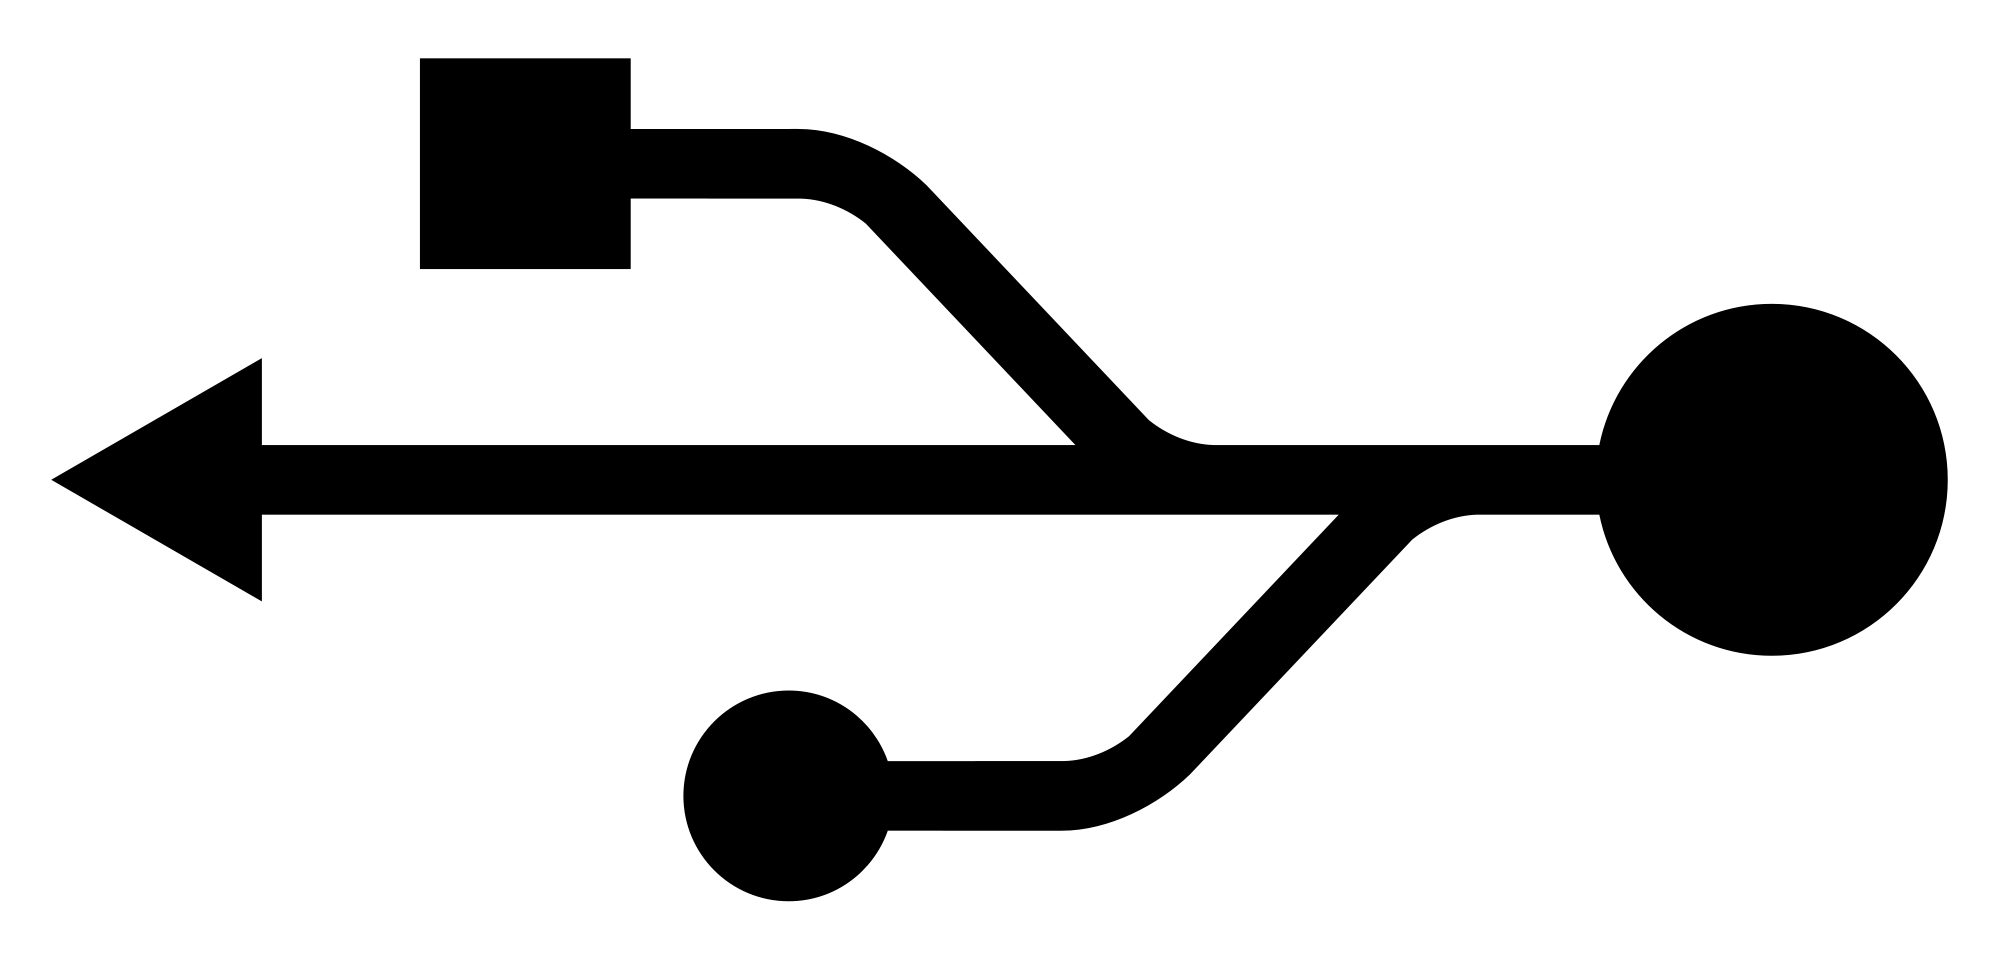
\includegraphics[width=5mm]{./figures/usb.png}};
			\node[draw,fill=gray!50,minimum height=6mm,minimum width=8mm,below=2pt of usb1](usb2) {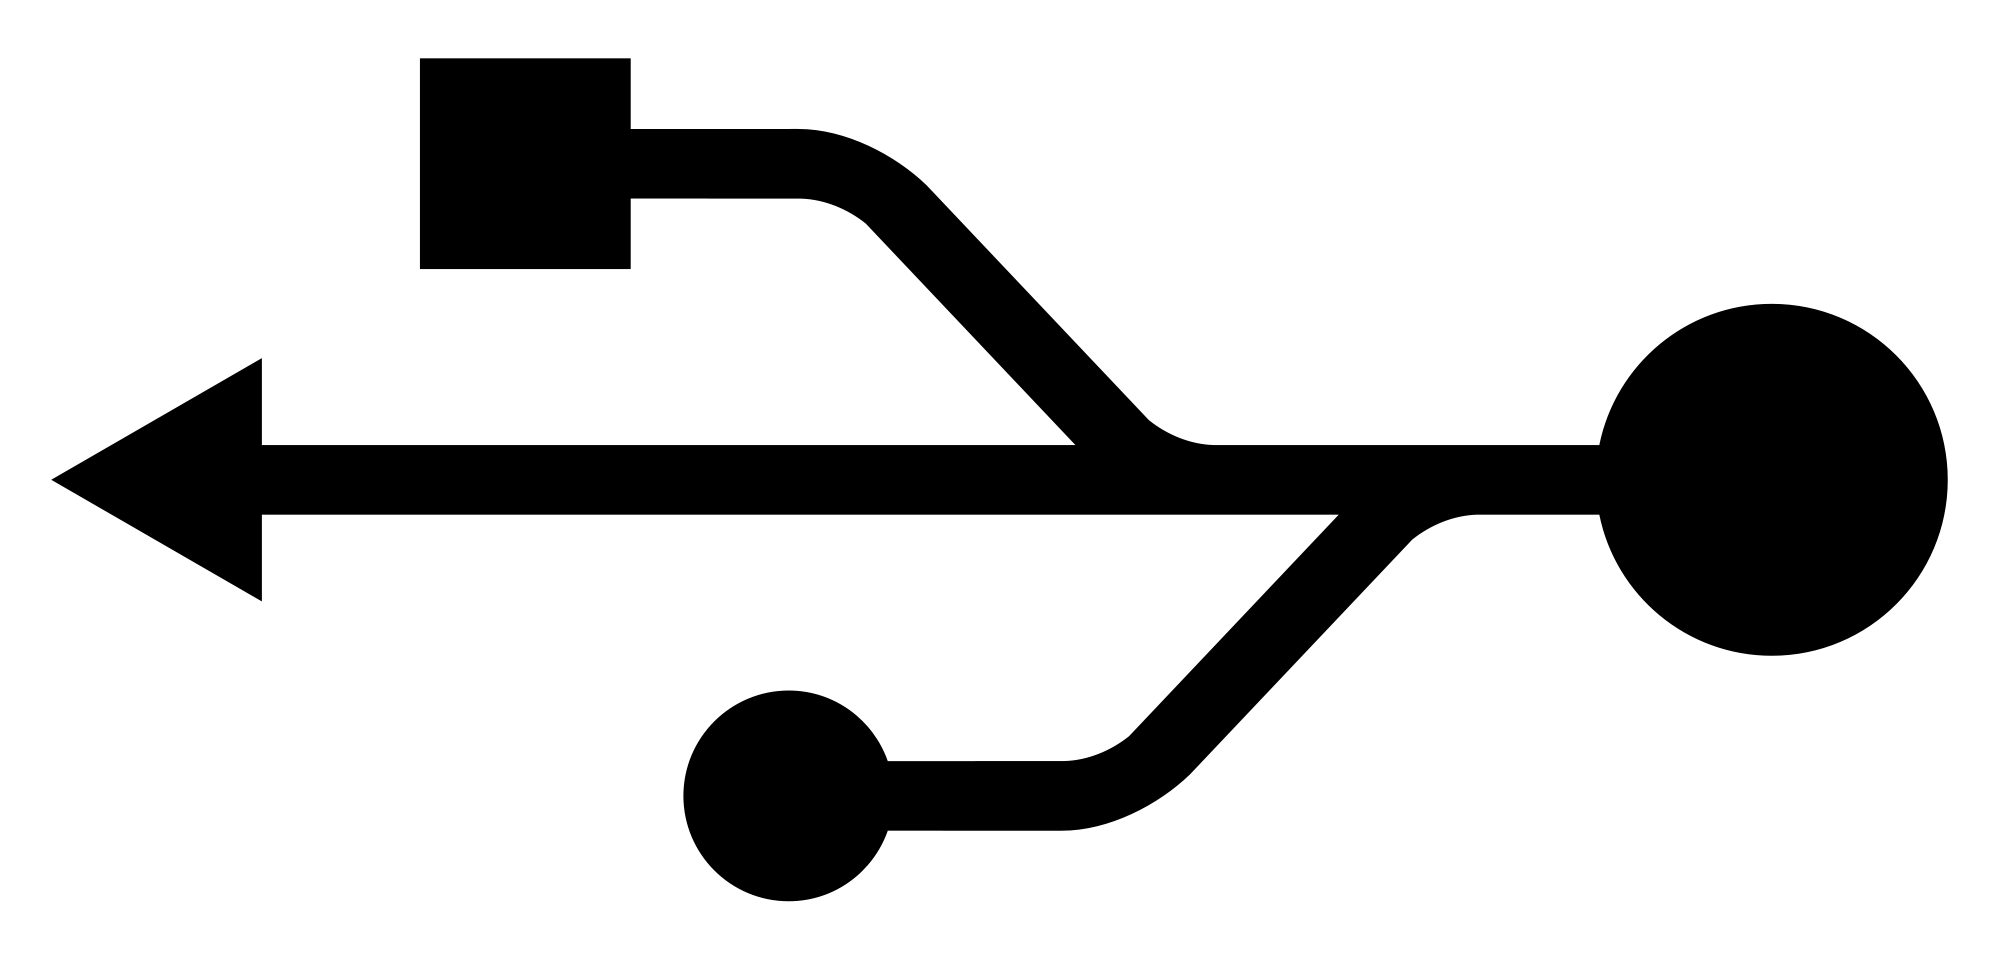
\includegraphics[width=5mm]{./figures/usb.png}};
			\node[draw,fill=gray!50,minimum height=3mm,minimum width=4mm,anchor=north east,xshift=-0.7cm](microusb) at (rpi.north east) {};
			\node[fill=black!80,minimum height=3mm,minimum width=20mm,anchor=south east,xshift=-2mm,yshift=2mm](gpio) at (rpi.south east) {};
				\node[right=0.1cm of gpio]{\footnotesize \scshape gpio};
			\foreach \position in {1,2,...,15}{
				\node[fill=yellow!60,circle,inner sep=0.5pt](pin\position) at ($(gpio.north west)+(\position/8,-1mm)$) {};
				\node[fill=yellow!60,circle,inner sep=0.5pt](pin\position+15) at ($(gpio.north west)+(\position/8,-2mm)$) {};
			}
		}

		\drawocas{}
		\drawuav{left=2.5cm of ocas,yshift=0.3cm}
		\drawgcs{left=2cm of ocas,yshift=3.5cm}
		\drawrpi{}

		% Wifi
		\node[fill,inner sep=0pt,minimum width=1mm,minimum height=6mm,above left=0.5cm of usb1](wifi-stick){};
		\node[circle,inner sep=0.7mm,fill,above=-1pt of wifi-stick](wifi-ball) {};
		\node[fit=(wifi-stick)(wifi-ball)](wifi) {};

		% Power
		\node[fill=black!50,minimum height=4mm,minimum width=7mm,above right=0.5cm of microusb](power) {\footnotesize Power};

		% Sonar
		\node[fill=blue!70,minimum height=5mm,minimum width=9mm,below=0.7cm of gpio,xshift=5mm](sonar-board){};
		\node[fill=black!80,draw=black!50,very thick,circle,inner sep=1mm,xshift=-2mm](sonar1) at (sonar-board) {};
		\node[fill=black!80,draw=black!50,very thick,circle,inner sep=1mm,xshift=2mm](sonar2) at (sonar-board) {};
		\node[fit=(sonar-board)(sonar1)(sonar2)](sonar){};


		% Connections (paths)
		\draw[semithick,decorate,decoration={coil,aspect=0,segment length=1.1cm}] (usb2.west) -- node[below=2mm,sloped]{MAVlink} (uav);
		\draw[semithick,decorate,decoration={expanding waves,angle=4,segment length=2mm}] (wifi-ball.north east) -- node[above=2mm,sloped]{SSH (WiFi)} (gcs);
		\draw[semithick] (usb1.west) -| (wifi-stick.south);
		\draw[semithick,double] (microusb) |- (power);
		\draw[semithick,decorate,decoration=zigzag] (sonar-board) -- (sonar-board|-gpio.south);
		%\foreach \wire in {-1.5,-0.5,0.5,1.5}
		%	\draw ($(sonar-board.north)+(\wire/20,0)$) -- ($(sonar-board.north|-gpio.south)+(\wire/20,0)$);

	\end{tikzpicture}

	\caption{OCAS hardware layout}
	\label{fig:ocas}
\end{figure}


\subsection{Power connection}
For the Raspberry Pi to boot up, the only requirement is to provide a continuous current of 5V and enough current to power any other peripheral as well as the board, which in any case will not be higher than 2A.
Thus, the battery pack, providing a continuous source of energy during during the whole duration of the mission is enough to meet the requirement.
It is connected to the Raspberry Pi SBC via a conventional USB type A, at the battery end, to micro-USB type B, at the computer end; no additional action being required.

\subsection{MAVlink connection}
The connection with the UAV (i.e. with the Ardupilot controller board) is done also via a regular USB cable, making use of the serial communications protocol.
The serial protocol is a simple manner of tranfering information which consists on transmitting the data one bit at a time, avoiding the synchronisation problem.
Hence, the only issue is that both ends must agree in advance on the transmission rate.
This is done by setting a common ``baud rate'', where a baud is the unit for symbol change (signal event) rate, commonly measured in bits per second.
In the particular case of communicating with the UAV, the messages transmitted through the serial link are defined according to the MAVlink protocol.

\subsection{GCS connection}
The link with the Ground Control Station is composed of two intermediate steps:

On one hand, the network adapter is connected to a USB port on the Raspberry Pi to provide the SBC with wireless networking capabilities.
This connection is entirely handled by the kernel, the adapter's drivers and the operating system, and needs no further action from the engineer.

The second step is decidedly more complex.
Firstly, the Raspberry Pi needs to be set up to wirelessly connect to the same network as the GCS computer.
There are several ways to achieve this goal, but an uncomplicated one is to create an ad-hoc network from the GCS computer (running Windows) to which the Raspberry Pi is directly connected.
The specific details are explained in Appendix \ref{app:network}.
This approach has been mainly chosen for its simplicity and portability, but notice that there exist more advanced network architectures that could provide significantly better performance.
Secondly, the SSH connection needs to be stablished over the network.
The process involves searching for the Raspberry Pi's address on the network, connecting to the SSH port and, optionally, setting up an X server for an easier Graphical User Interface (GUI) with the OCAS.
More details on the steps to be taken are developed in Appendix \ref{app:ssh}.

\subsection{GPIO connection}

The General Purpose Input / Output pins on the Raspberry Pi operate on a notably lower level than the previous hardware connections.
As their name implies, the GPIO pins are the most general type of connection the Raspberry Pi can handle.
The reason is that these pins have to be manually operated; that is, each of the pins can be set via software to either a HIGH or LOW state, meaning 3.3V or 0V with respect to the Ground (GND) potential, respectively.

Hence, in this project, the GPIO pins will be used to both trigger the ultrasonic rangefinders and read the returning signal that encodes the information on the distance from the sensor to the detected obstacle.

Besides, the sonar is equipped with its own microcontroller, which handles the lowest-level signals.
For its operation, it counts with 4 different pins (see Figure \ref{fig:hc-sr04}) 
\begin{enumerate}
	\item GND, or Ground, specifies the reference voltage of the device.
	\item VCC, which stands for Voltage Continuous Current, powers the sensor at 5V.
	\item Trigger is an input signal pin.
		A HIGH value on this pin triggers (hence the name) a series of short bursts of sound from the piezoelectric speaker, which will rebound on any close obstacle.
	\item Echo is the output signal pin.
		The sensor's microcontroller processes the sound captured by the microphone and sends a short pulse through the echo pin exactly after the rebounded sound signal is received.
		Knowing the speed of propagation of sound (given by $a=\sqrt{\gamma R_g T}$) and the time taken for the wave to travel to the obstacle and back, the distance can be calculated with $d=v \cdot t/2$
\end{enumerate}
The ultrasonic rangefinder's technical documentation can be found in Appendix \ref{app:sonar-doc}.

On the Raspberry Pi side, the VCC pin shall be connected to any 5V pin, the GND pin to a Ground pin, and the Trigger and Echo pins to any numbered GPIO pins, depicted in Figure \ref{fig:gpio}.


\begin{figure}[htbp]
	\centering
	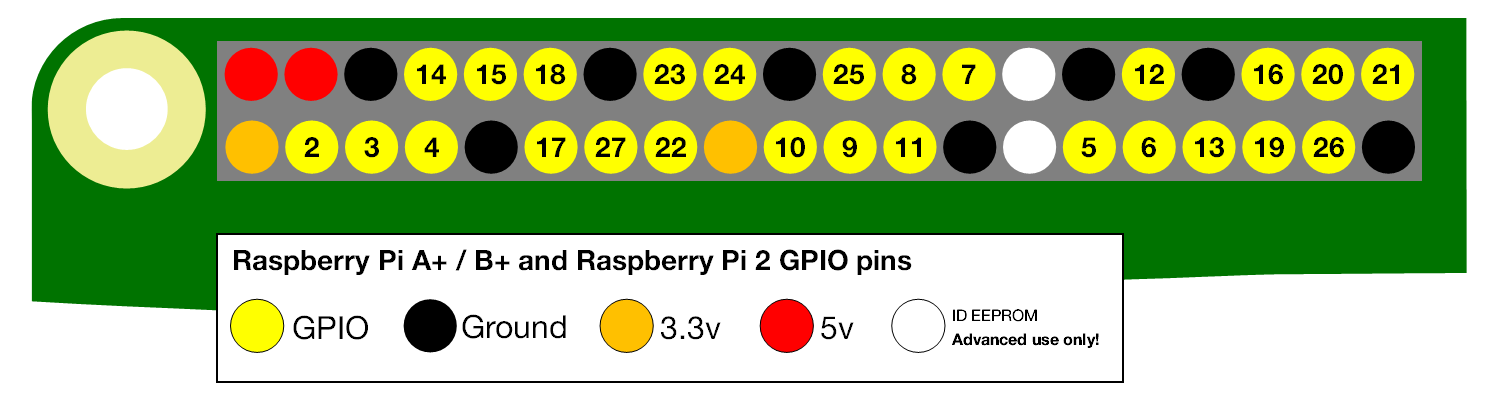
\includegraphics[width=0.6\textwidth]{./figures/gpio.png}
	\caption{GPIO pins on the Raspberry Pi 2 model B {\footnotesize Source: \url{raspberrypi.org}}}
	\label{fig:gpio}
\end{figure}


There is one important issue that needs to be noticed, though.
The rangefinders work on 5V only and, while the Raspberry Pi can provide 5V to power the sensors, the GPIO pins can be damaged if operated at more than 3.3V.
Thus, the signal pins must be reduced from 5V to 3.3V before being connected to the SBC.
The solution to the problem is to use a ``voltage divider'', which is a passive circuit that outputs a fraction of the input voltage by means of a pair of resistors, which are connected as shown in Figure \ref{fig:voltage}.

\begin{figure}[htbp]
	\centering
	\begin{tikzpicture}[circuit ee IEC,large circuit symbols]

		%\node[ground,point down,info={GND}](gnd){};	
		%\node[resistor,point up,info={R$_1$},right of=gnd](r1){};
		%\coordinate[above of=r1](coord);
		%\node[resistor,point up,info={R$_2$},right of=coord](r2){};
		%\node[contact,info={V$_{in}$},above left of=r2,yshift=0.4cm](vin){};
		%\node[contact,info={V$_{out}$},right of=coord](vout){};

		%\draw (vin) -| (r2) to (coord) to (vout) to (coord) to (r1) to (gnd);

		\node[ground,info=GND](gnd){};	
        \node[resistor,info=R$_2$,left=1 of gnd](r2){};
        \coordinate[left of=r2](coord);
        \node[resistor,info=R$_1$,left of=coord](r1){};
        \node[contact,info=left:V$_{in}$,above left of=r1,xshift=-10](vin){};
		\node[contact,info=left:V$_{out}$,below of=coord](vout){};

		\draw (vin) |- (r1) to (coord) to (vout) to (coord) to (r2) to (gnd);
		
	\end{tikzpicture}
	\caption{Schematic of a voltage divider}
	\label{fig:voltage}
\end{figure}


In the present case, for the voltage to drop from 5V to 3.3V, the resistors need to meet:
\begin{equation}
	\frac{V_{in}}{R_1+R_2}=\frac{V_{out}}{R_2} \ \Rightarrow\ \frac{V_{in}}{V_{out}}=\frac{R_1}{R_2}+1 \ \Rightarrow\ \frac{R_1}{R_2}=\frac{5V}{3.3V}-1 \ \Rightarrow\ \frac{R_1}{R_2}=\frac{1}{2} 
\end{equation}

So finally, an ultrasonic rangefinder connected to GPIO pins 14 and 15, for instance, would be connected a shown in Figure \ref{fig:sonarconnect}.

\begin{figure}[htbp]
	\centering
	\begin{tikzpicture}

		\node(rpi){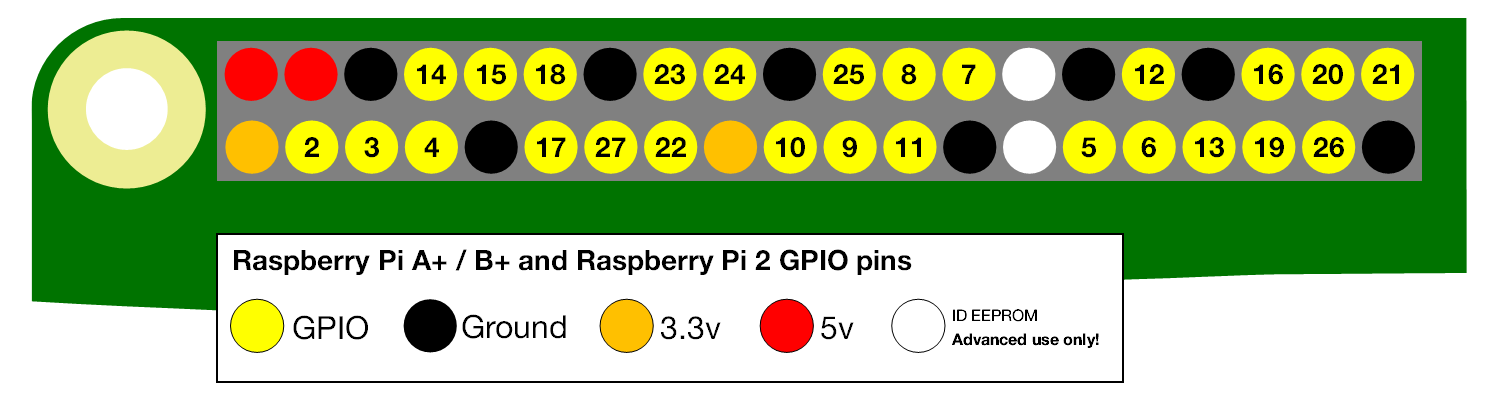
\includegraphics[width=0.5\textwidth,trim={0 6cm 0 0},clip]{./figures/gpio.png}};
		\node[above=15mm of rpi,xshift=-1.2cm](sonar){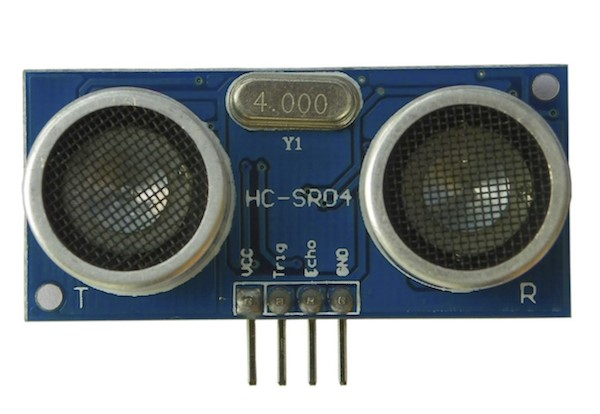
\includegraphics[width=0.2\textwidth,trim={0 2mm 0 2mm},clip]{./figures/hc-sr04.jpg}};

		\coordinate(VCC) at ($(sonar.south)+(-2.7mm,4mm)$);
		\coordinate(TRIG) at ($(sonar.south)+(-1.1mm,4mm)$);
		\coordinate(ECHO) at ($(sonar.south)+(0.7mm,4mm)$);
		\coordinate(GND) at ($(sonar.south)+(2.3mm,4mm)$);

		\coordinate(v) at ($(sonar.south)+(-2.7mm,0)$);
		\coordinate(t) at ($(sonar.south)+(-1.1mm,-2mm)$);
		\coordinate(e) at ($(sonar.south)+(0.7mm,-7mm)$);
		\coordinate(g) at ($(sonar.south)+(2.3mm,-15mm)$);

		\coordinate(vcc) at ($(rpi.north west)+(17.6mm,-5.7mm)$);
		\coordinate(gnd) at ($(rpi.north west)+(20.8mm,-5.7mm)$);
		\coordinate(trig) at ($(rpi.north west)+(24.0mm,-5mm)$);
		\coordinate(echo) at ($(rpi.north west)+(27.0mm,-5mm)$);

		\node[draw,fill=white,minimum width=2mm,minimum height=5mm,inner sep=0,above=2mm of e](r1){\tiny R$_1$};
		\node[draw,fill=white,minimum width=2mm,minimum height=5mm,inner sep=0,above=7mm of gnd](r2){\tiny R$_2$};

		\draw[line width=0.5mm,blue!50] (e) -| (r2);
		\draw[line width=0.5mm,blue!50] (r2) -- (gnd);

		\draw[line width=0.5mm,red] (VCC) -- (v) -| (vcc);
		\draw[line width=0.5mm,black] (GND) -- (g) -| (gnd);
		\draw[line width=0.5mm,green!80] (TRIG) -- (t) -| (trig);
		\draw[line width=0.5mm,blue!80] (ECHO) -- (r1);
		\draw[line width=0.5mm,blue!80] (r1) -- (e) -| (echo);
		
		\node[fill=blue!80,circle,inner sep=0.4mm,above=12.3mm of echo] (connEcho){};
		\node[fill=black,circle,inner sep=0.4mm,above=5mm of gnd] (connGnd){};

	\end{tikzpicture}
	\caption{Connection of the HC-SR04 sensor to the Raspberry Pi}
	\label{fig:sonarconnect}
\end{figure}



\section{Software: Bringing everything together}

Having several flows of information arriving to the Raspberry Pi, it is crucial to set up a system that acquires all the data before it can be processed. 
In the present section such a system will be described.

\subsection{The Operating System}

The first software layer on the Raspberry Pi (apart from the kernel) is the Operating System (OS).
In this case, the linux OS is Raspbian Wheezy, which is a version of Debian adapted to be run on the Raspberry Pi's ARMv7 chip.

Raspbian is a complete OS, and as such its abilities are varied, being the most relevant for the project the network management tools and the capability of running external software applications.
Within the OCAS, Raspbian will be used as container of the software subsystems specified in the Logical Decomposition phase of the design process (Figure \ref{fig:pbs}), plus it will directly handle the functions associated to the GCS connector.
An schematic of the relevant software architecture to the OCAS is represented in Figure \ref{fig:software}.

\begin{figure}[htbp]
	\centering
	\begin{tikzpicture}

		\newcommand{\drawrpi}[1]{
			\node[#1,fill=green!70!black,minimum height=6cm,minimum width=10cm,rounded corners=2mm](rpi) {};
			\coordinate[label=above right:\textcolor{white}{RPi}]
				(rpi-label) at (rpi.south west) {};
			\node[draw,fill=gray!50,minimum height=6mm,minimum width=8mm,anchor=north west,yshift=-2pt](usb1) at (rpi.north west) {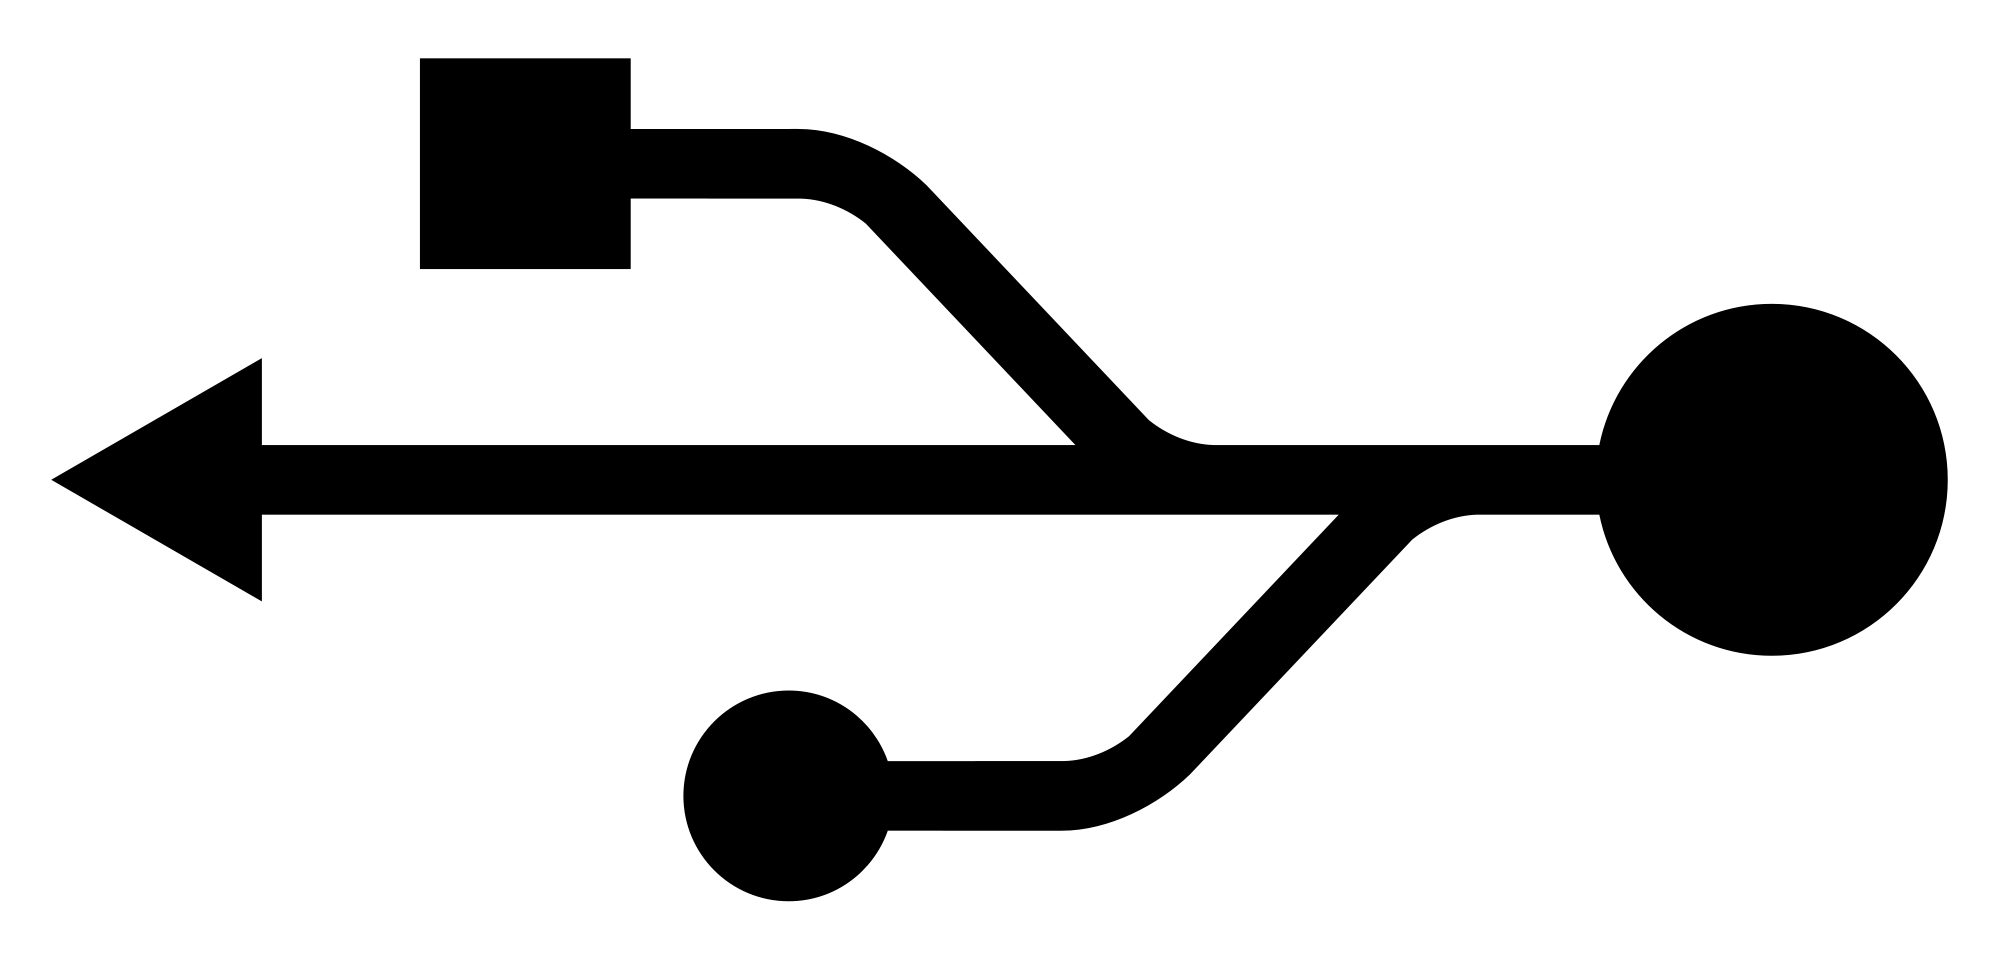
\includegraphics[width=5mm]{./figures/usb.png}};
			\node[draw,fill=gray!50,minimum height=6mm,minimum width=8mm,below=2pt of usb1](usb2) {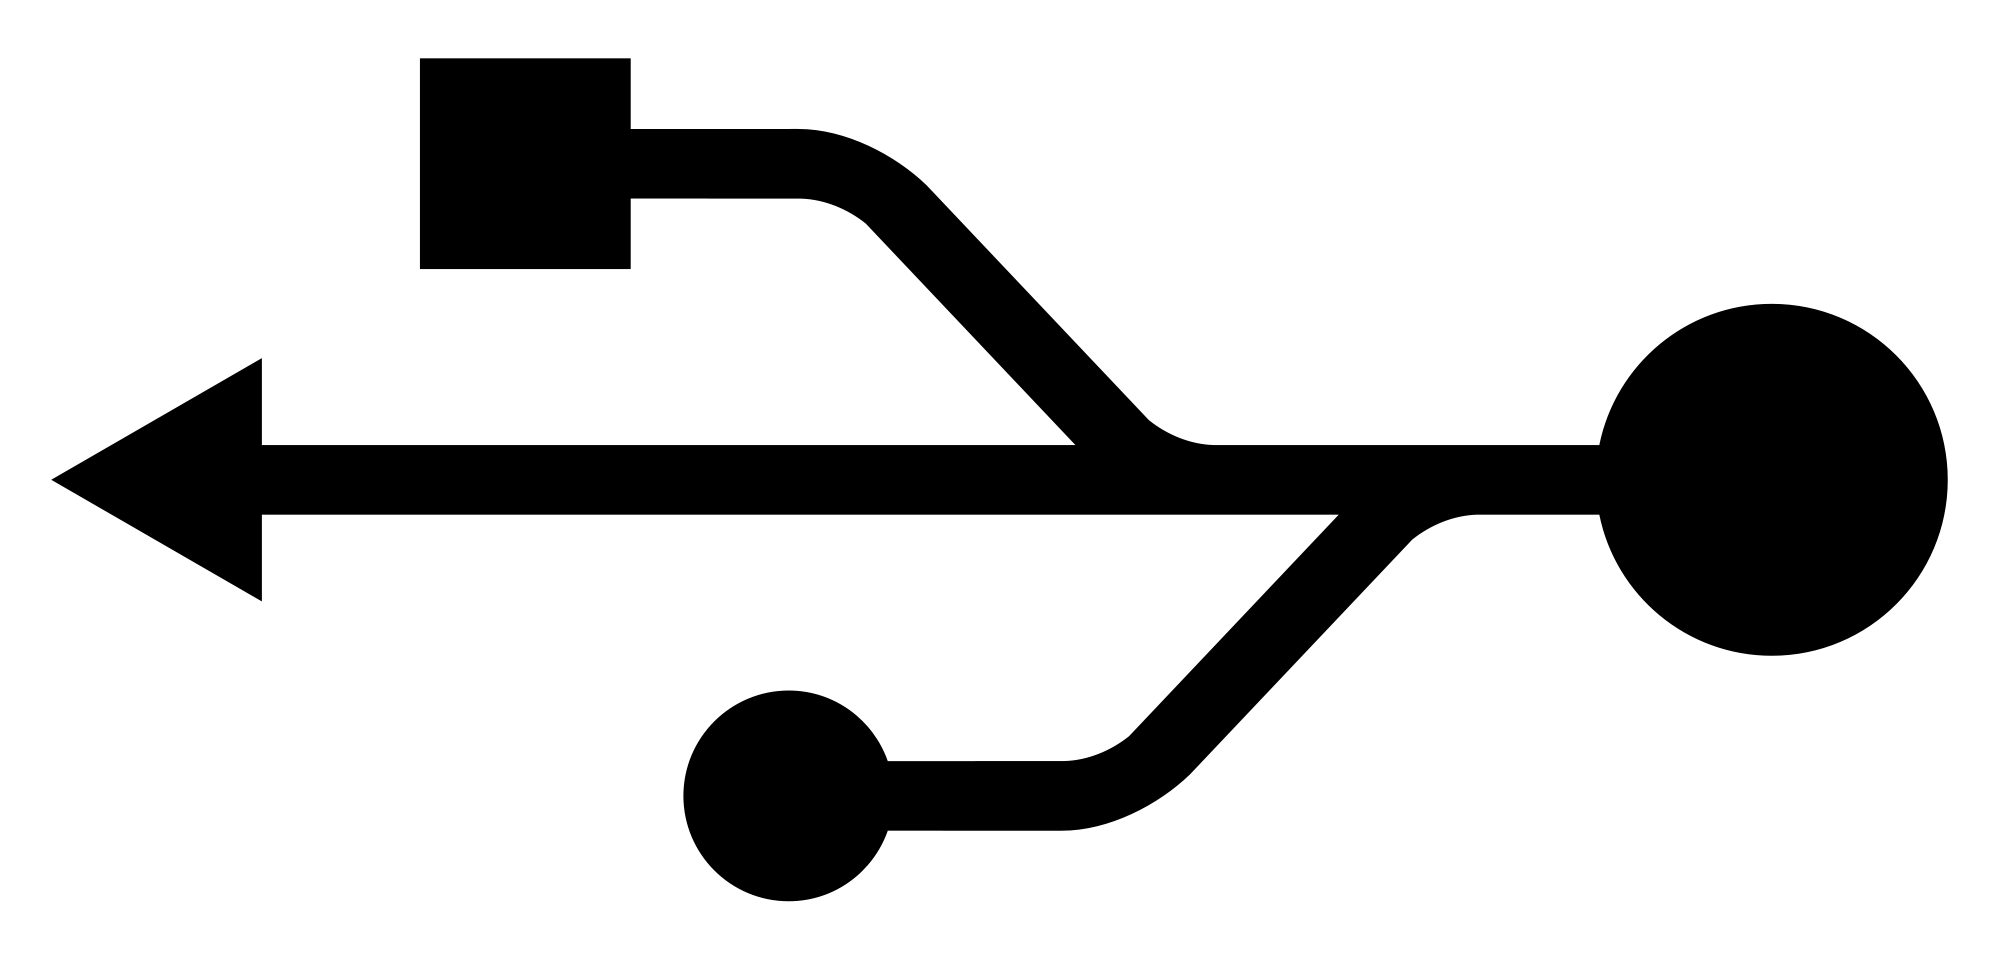
\includegraphics[width=5mm]{./figures/usb.png}};
			\node[draw,fill=gray!50,minimum height=3mm,minimum width=4mm,anchor=north east,xshift=-0.7cm](microusb) at (rpi.north east) {};
			\node[fill=black!80,minimum height=3mm,minimum width=20mm,anchor=south east,xshift=-2mm,yshift=2mm](gpio) at (rpi.south east) {};
				%\node[right=0.1cm of gpio]{\footnotesize \scshape gpio};
			\foreach \position in {1,2,...,15}{
				\node[fill=yellow!60,circle,inner sep=0.5pt](pin\position) at ($(gpio.north west)+(\position/8,-1mm)$) {};
				\node[fill=yellow!60,circle,inner sep=0.5pt](pin\position+15) at ($(gpio.north west)+(\position/8,-2mm)$) {};
			}
		}

		\newcommand{\drawgcs}[1]{
			\node[rectangle,rounded corners=3pt,double,draw=gray,thick,minimum height=0.3cm,minimum width=0.5cm,#1](display){\footnotesize GCS};
			\node[trapezium,rounded corners=2pt,draw=gray,very thick,trapezium angle=50,minimum height=0.1cm,inner ysep=1pt,inner xsep=3mm,below=2pt of display](keyboard){};

			\node[fit=(display)(keyboard),inner sep=0mm] 
				(gcs) {};	%Group the GCS together
		}

		\newcommand{\drawuav}[1]{
			\node[#1](coord){};
			\coordinate[fill=gray,draw=gray,circle,minimum size=0.1cm,inner sep=0] (m1) at ($(coord)+(-0.4cm,0.4cm)$) {};
			\coordinate[fill=gray,draw=gray,circle,minimum size=0.1cm,inner sep=0] (m2) at ($(coord)+(0.4cm,0.4cm)$) {};
			\coordinate[fill=gray,draw=gray,circle,minimum size=0.1cm,inner sep=0] (m3) at ($(coord)+(0.4cm,-0.4cm)$) {};
			\coordinate[fill=gray,draw=gray,circle,minimum size=0.1cm,inner sep=0] (m4) at ($(coord)+(-0.4cm,-0.4cm)$) {};

			%Airframe
			\path[fill=gray,draw=gray,line width=0.7mm] (m1.center)
				.. controls (coord) .. (m2.center)
				.. controls (coord) .. (m3.center)
				.. controls (coord) .. (m4.center)
				.. controls (coord) .. (m1.center);
				

			%Propellers
			\path[fill=gray] (m1) arc (155:115:0.5cm) arc (335:295:0.5cm)
				arc (115:155:0.5cm) arc (295:335:0.5cm);
			\path[fill=gray] (m2) arc (65:25:0.5cm) arc (245:205:0.5cm)
				arc (25:65:0.5cm) arc (205:245:0.5cm);
			\path[fill=gray] (m3) arc (155:115:0.5cm) arc (335:295:0.5cm)
				arc (115:155:0.5cm) arc (295:335:0.5cm);
			\path[fill=gray] (m4) arc (65:25:0.5cm) arc (245:205:0.5cm)
				arc (25:65:0.5cm) arc (205:245:0.5cm);

			\node[yshift=-0.8cm](uav-label) at (coord) {\footnotesize UAV};

			\node[fit=(coord)(m1)(m2)(m3)(m4)(uav-label),inner sep=1.4mm]
				(uav) {};	%Group the UAV together
		}

		\newcommand{\drawsensor}[1]{
			\node[#1,fill=blue!70,minimum height=5mm,minimum width=9mm](sonar-board){};
			\node[fill=black!80,draw=black!50,very thick,circle,inner sep=1mm,xshift=-2mm](sonar1) at (sonar-board) {};
			\node[fill=black!80,draw=black!50,very thick,circle,inner sep=1mm,xshift=2mm](sonar2) at (sonar-board) {};
			\node[fit=(sonar-board)(sonar1)(sonar2),inner sep=0](sonar){};
		}

		\newcommand{\drawos}[1]{
			\node[#1,fill=brown,minimum height=4.5cm,minimum width=7cm](os){};
			\coordinate[label=above right:\textcolor{white}{Raspbian}]
				(raspbian-label) at (os.south west) {};
			\node[fill=brown!80!black,anchor=north west,align=left,inner sep=2mm](network) at (os.north west) {Network tools\\ SSH client};
			%\node[rectangle,right=1cm of network](shell) {Unix shell};
			\node[fill=yellow!90!black,rounded corners,anchor=south east,minimum height=2.7cm,minimum width=4.6cm](python) at ($(os.south east)+(-3mm,3mm)$) {};
			\coordinate[label=above right:\textcolor{white}{Python}]
				(python-label) at (python.south west) {};
			\node[anchor=north west](gui) at ($(python.north west)+(6mm,-2mm)$) {GUI};
			\node[anchor=west](mavproxy) at ($(python.west)+(1mm,-2mm)$) {MAVproxy};
			\node[anchor=north east,align=right](script) at ($(python.north east)+(-3mm,-2mm)$) {Control\\ script};
		}


		\begin{scope}[transparency group,opacity=0.4]
			\drawrpi{}
			\drawgcs{left=of usb1,yshift=1mm}
			\drawuav{below left=of usb2,xshift=-3mm}
			\drawsensor{right=of gpio}
		\end{scope}
		\drawos{}

		\coordinate (mav) at ($(mavproxy)+(-3.5cm,0)$);

		\draw[thick,decorate,decoration={expanding waves,angle=10,segment length=0.8mm}] (usb1) -- node[above=2mm,sloped]{SSH} (gcs);
		\draw[thick,rounded corners] (usb1) -| (network);
		\draw[thick,rounded corners,-stealth] (network) |- node[fill=brown,align=center,inner sep=0,opacity=0.8](shell){\small Unix\\[-1ex] \small shell} (gui);

		\draw[thick,decorate,decoration={coil,aspect=0,amplitude=0.5mm,segment length=0.5cm}] (usb2) -| node[below right=1.5mm]{MAVlink} (uav) ;
		\draw[thick,decorate,decoration={coil,aspect=0,amplitude=0.5mm,segment length=0.5cm}] (mavproxy) -- (mav) |- (usb2) ;
		\draw[thick,-stealth] (gui) -- (script.west|-gui);
		\draw[thick,-stealth] (gui) -- (mavproxy);
		\draw[thick,decorate,decoration={coil,aspect=0,amplitude=0.5mm,segment length=0.3cm,pre length=5pt,post length=3pt},stealth-stealth] ($(mavproxy.north east)+(-3mm,-1mm)$) -- ($(script.south west)+(3mm,4mm)$);

		\draw[thick,decorate,decoration=zigzag] (sonar) -- (gpio);
		\draw[thick,decorate,decoration=zigzag,-stealth] (gpio) -| (script);

		
	\end{tikzpicture}
	\caption{Software architecture of the OCAS computer}
	\label{fig:software}
\end{figure}


As it can be deduced from Figure \ref{fig:software}, all the interaction from the Ground Control Station to the OCAS computer is performed through the Unix Shell, which only provides a command interface with the user.
Nevertheless, the SSH connection allows an optional X Window System protocol forwarding (as mentioned in Section \ref{sec:ocasintegration}); and a Graphical User Interface (GUI) will be developed in response to Requirement 8.1, allowing the execution of MAVproxy as well as the custom control scripts in order to enhance the intuitive operation of the system by the pilot.

\subsection{MAVproxy} \label{sec:mavproxy}

MAVproxy is an open-source Ground Control Station piece of software that is distributed as a Python application.
Thus, it can be run on any machine on which a Python distribution can be installed (virtually any operating system).

Its most significant difference compared with traditional GCS software such as Mission Planner or QGroundControl is that MAVproxy is built for the command line and does not need a graphical desktop environment to operate (although a small state window and map are also implemented), which means that it is the most adequate alternative for the operation of the UAV from the OCAS.
Furthermore, another decisive feature is the ability of MAVproxy of forwarding the MAVlink messages that are received from and sent to the UAV, allowing the possibility of operating as an intermediate software layer between the UAV and other GCS pieces of software.
That in particular is the chosen architecture for the OCAS in terms of communication between the UAV and the custom control scripts, which will be covered in Section \ref{sec:script}.

Concerning the present section, the setup of MAVproxy will be explained.

\begin{figure}[htbp]
	\centering
	\begin{tikzpicture}
		
		\newcommand{\drawuav}[1]{
			\node[#1](coord){};
			\coordinate[fill=gray,draw=gray,circle,minimum size=0.1cm,inner sep=0] (m1) at ($(coord)+(-0.4cm,0.4cm)$) {};
			\coordinate[fill=gray,draw=gray,circle,minimum size=0.1cm,inner sep=0] (m2) at ($(coord)+(0.4cm,0.4cm)$) {};
			\coordinate[fill=gray,draw=gray,circle,minimum size=0.1cm,inner sep=0] (m3) at ($(coord)+(0.4cm,-0.4cm)$) {};
			\coordinate[fill=gray,draw=gray,circle,minimum size=0.1cm,inner sep=0] (m4) at ($(coord)+(-0.4cm,-0.4cm)$) {};

			%Airframe
			\path[fill=gray,draw=gray,line width=0.7mm] (m1.center)
				.. controls (coord) .. (m2.center)
				.. controls (coord) .. (m3.center)
				.. controls (coord) .. (m4.center)
				.. controls (coord) .. (m1.center);
				

			%Propellers
			\path[fill=gray] (m1) arc (155:115:0.5cm) arc (335:295:0.5cm)
				arc (115:155:0.5cm) arc (295:335:0.5cm);
			\path[fill=gray] (m2) arc (65:25:0.5cm) arc (245:205:0.5cm)
				arc (25:65:0.5cm) arc (205:245:0.5cm);
			\path[fill=gray] (m3) arc (155:115:0.5cm) arc (335:295:0.5cm)
				arc (115:155:0.5cm) arc (295:335:0.5cm);
			\path[fill=gray] (m4) arc (65:25:0.5cm) arc (245:205:0.5cm)
				arc (25:65:0.5cm) arc (205:245:0.5cm);

			\node[yshift=-0.8cm](uav-label) at (coord) {\footnotesize UAV};

			\node[fit=(coord)(m1)(m2)(m3)(m4),inner sep=1.4mm]
				(uav) {};	%Group the UAV together
		}

		\tikzset{node distance=2cm}

		\drawuav{}
		\node[draw,fill=gray!50,minimum height=6mm,minimum width=8mm,right=3cm of uav](usb) {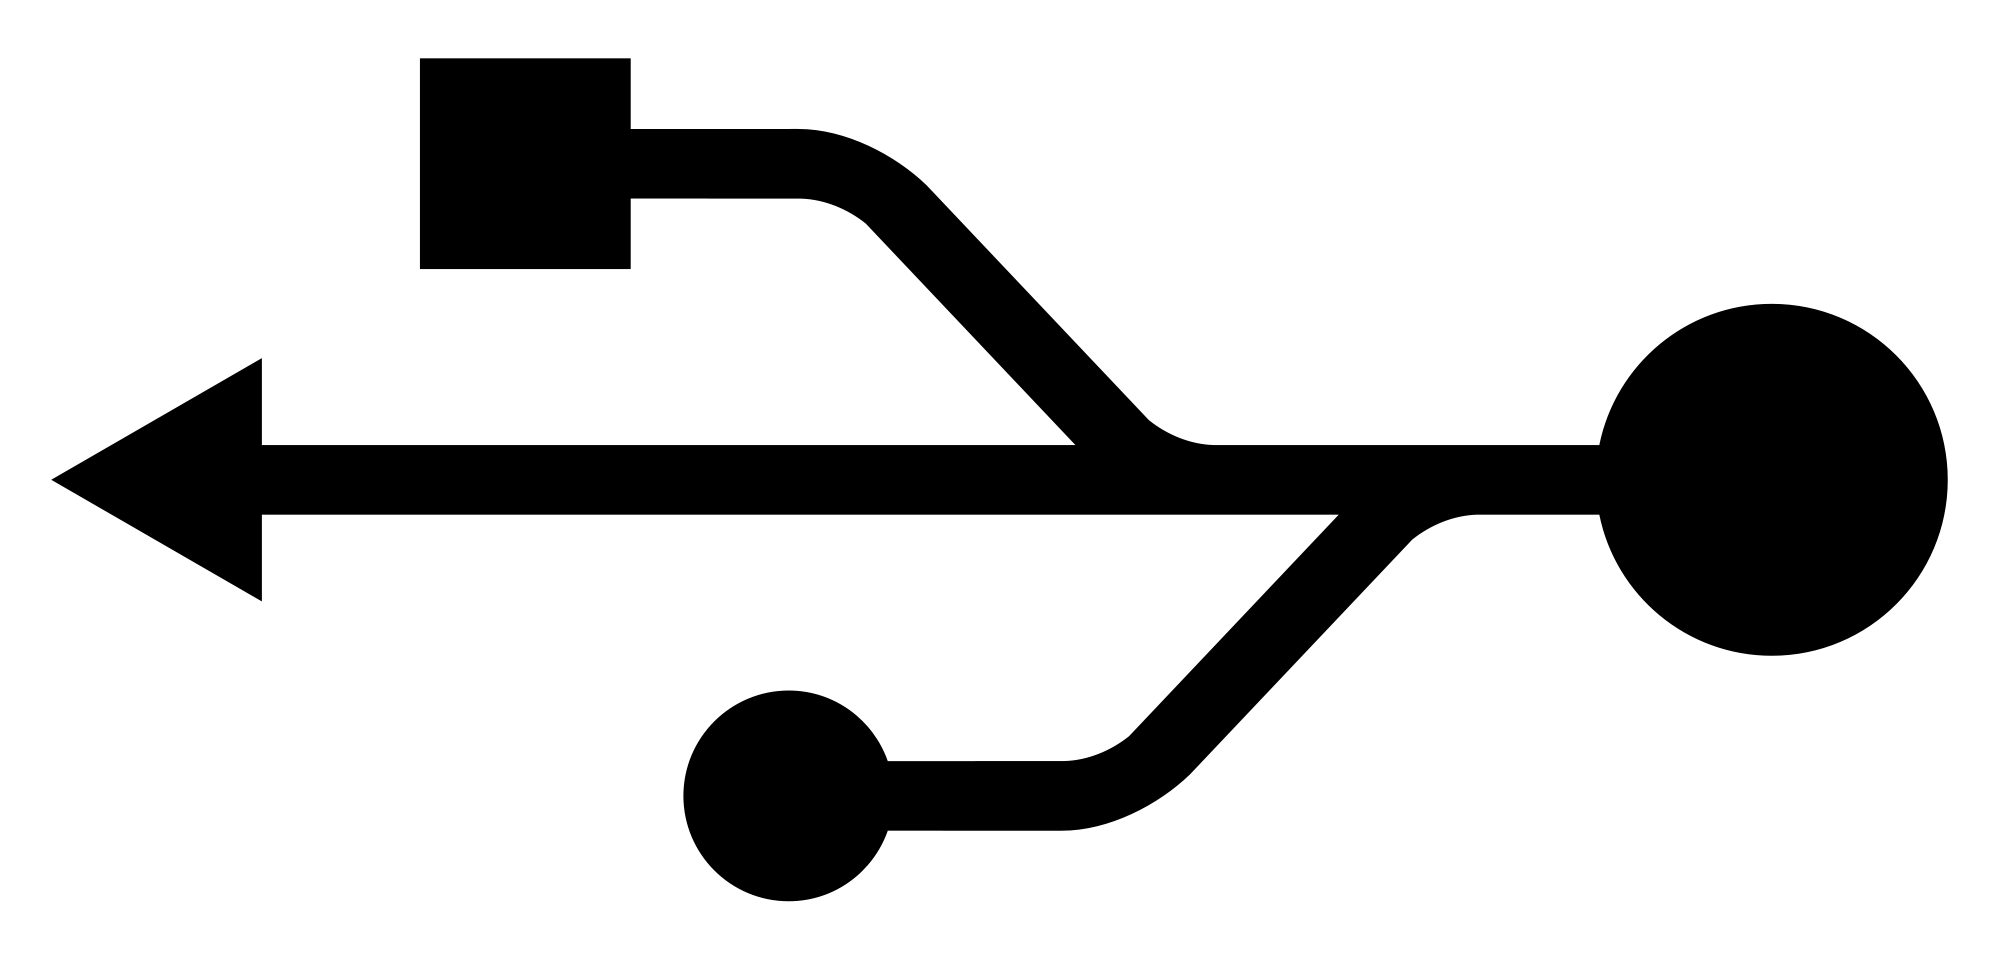
\includegraphics[width=5mm]{./figures/usb.png}};
			\node[below=0pt of usb]{\footnotesize /dev/ttyUSB0};
		\node[ellipse,draw,double,thick,inner sep=2mm,right=of usb](mavproxy){MAVproxy};
		\node[draw,rounded corners,below=1cm of mavproxy](window){State window};
		\node[draw,rounded corners,above=1cm of mavproxy](map){Map};
		\node[draw,semithick,minimum width=2cm,minimum height=1.5cm,above right=5cm of mavproxy,yshift=-3cm,align=center](script){Custom\\ control\\ script};
		\node[draw,semithick,minimum width=2cm,minimum height=1.5cm,below right=5cm of mavproxy,yshift=3cm,align=center](gcs){Other GCS\\ software};

		\draw[thick,stealth-stealth] (uav) -- node[above]{\footnotesize Serial comm.} (usb);
		\draw[thick,stealth-stealth] (usb) -- (mavproxy);
		\draw[thick,stealth-stealth] (mavproxy) -- node[above,sloped]{\footnotesize UDP: 127.0.0.1:14550} (script);
	\draw[thick,stealth-stealth] (mavproxy) -- node[below,sloped]{\footnotesize UDP: --.--.--.--:---} (gcs);
		\draw[-stealth] (mavproxy) -- (map);
		\draw[-stealth] (mavproxy) -- (window);


	\end{tikzpicture}
	\caption{MAVproxy setup}
	\label{fig:mavproxy}
\end{figure}


As previously mentioned and shown in Figure \ref{fig:mavproxy}, the connection from the UAV to the Raspberry Pi is done via a serial communication through USB cable.
The Ardupilot software utilises a baud rate of 115200 bd/s by default, which is an important parameter that needs to be specified to MAVproxy before connecting to the vehicle (else the connection will fail).
In addition, the address given by the OS to the USB port (/dev/ttyUSB0 in Figure \ref{fig:mavproxy}) has to be provided too. 

Finally, the redirection of MAVlink messages is done via the User Datagram Protocol (UDP), making use of the Internet Transport Layer.
However, a remote Internet connection is not needed, since both MAVproxy and the intended target (the custom control script) will be running on the same machine; hence the local IP address can be used (127.0.0.1) together with any available port of choice.
The optional second rerouting path is to be defined at the operator's discretion, and can be either a local or remote address.

The auxiliary Map and State windows are internally created by MAVproxy, using only Python function calls and libraries.

For completeness, the command to be executed in order to run the MAVproxy GCS software with the mentioned settings is:
\begin{center}
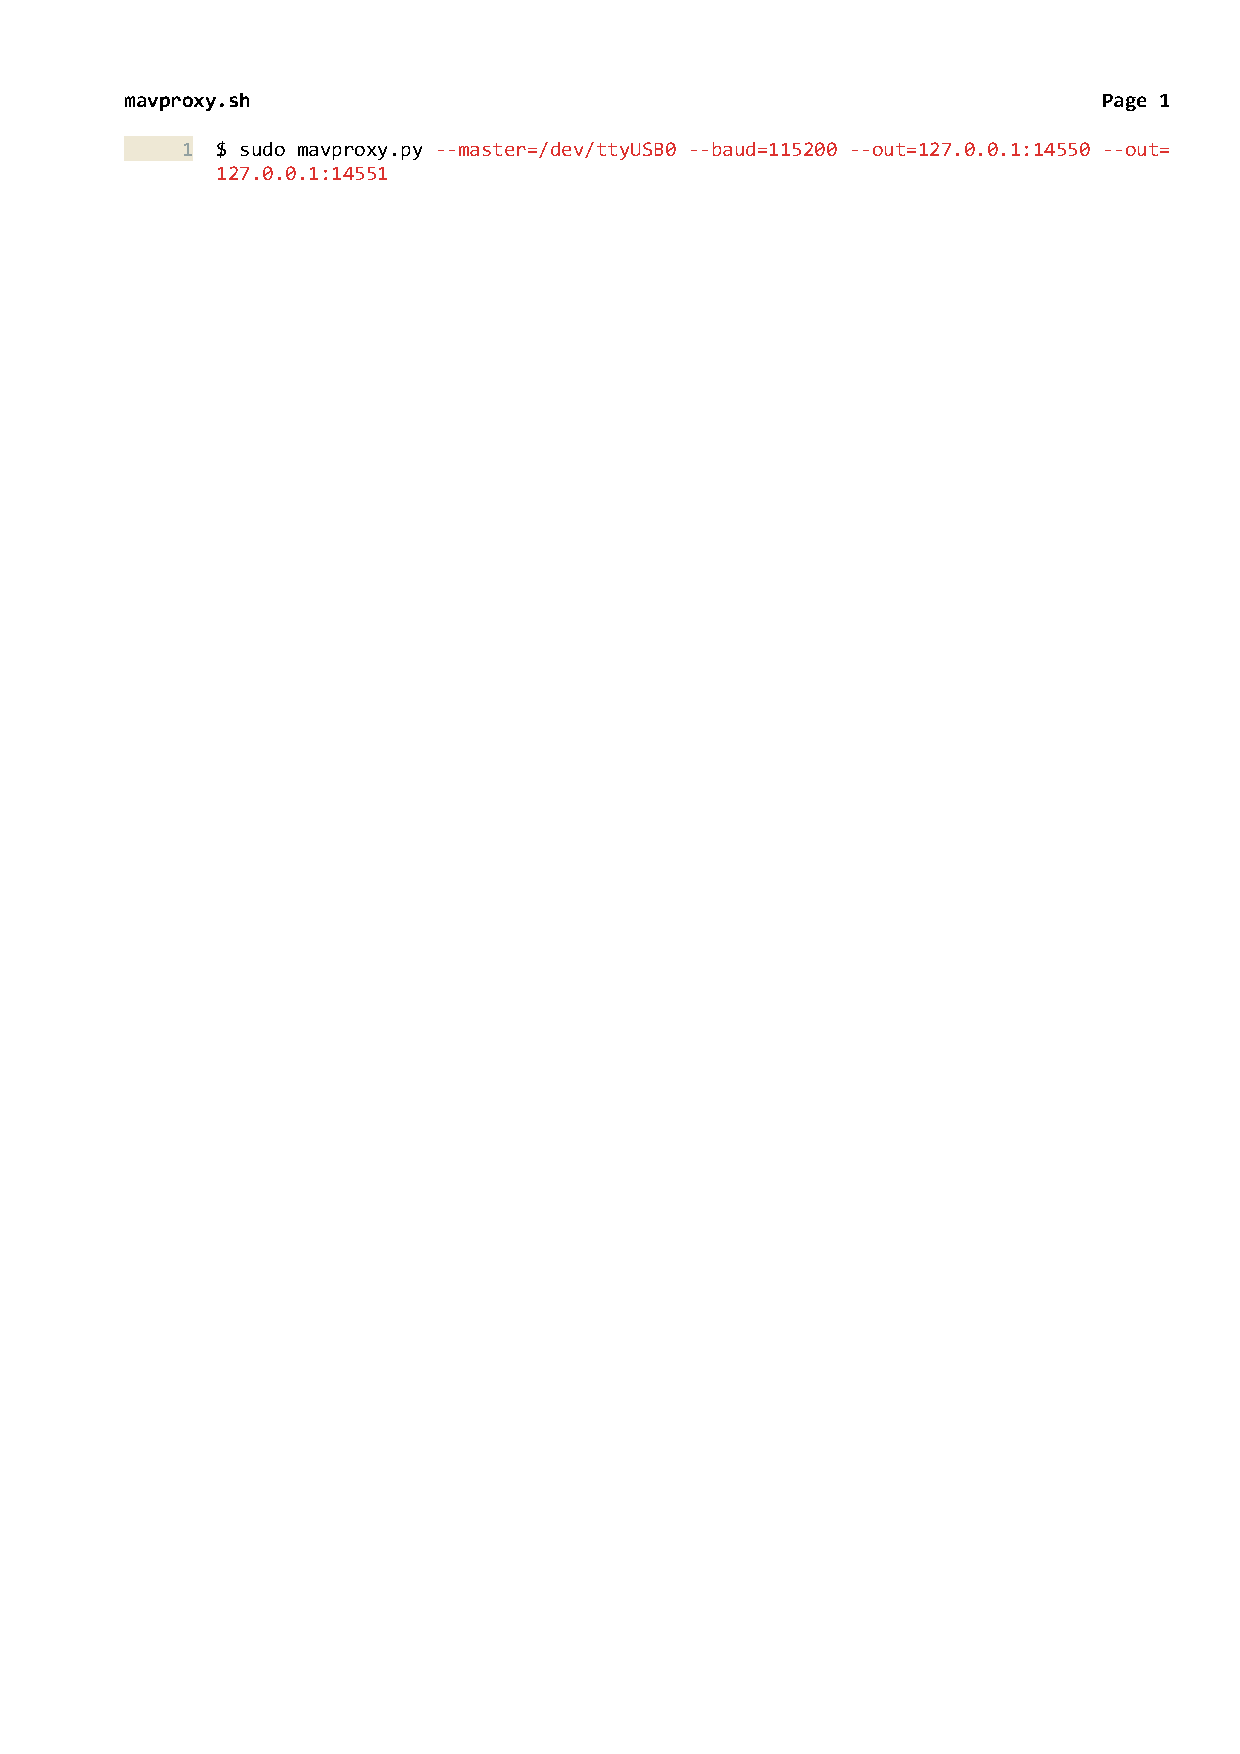
\includegraphics[width=0.9\textwidth,clip,trim={2.5cm 26.6cm 1cm 2.3cm}]{./figures/mavproxysh.pdf}
\end{center}

%\begin{lstlisting}[language=bash,basicstyle=\ttfamily\small,breaklines=true,breakatwhitespace=true,escapeinside={(*@}{@*)}]
%	(*@\textbf{\$}@*) sudo ./mavproxy.py --master=/dev/ttyUSB0 --baud=115200 --out=127.0.0.1:14550 --out=127.0.0.1:14551
%\end{lstlisting}

\subsection{The Python environment}

Python is an open-source general-purpose programming language built to be powerful and easy to use.
Additionally, it is implemented to run on virtually any machine, providing interpreters and compilers for most of the operating systems available, which means that the source code can be seamlessly ported from one system to another without any modifications to the source code.
Furthermore, Python has a considerable community of developers that contribute to the development of the language through a vast repository of libraries which allow for a greater abstraction and automation of common tasks.

These features and flexibility of Python make it ideal for the development of the OCAS.
In particular, there exists a community of developers leaded by 3D Robotics who are creating an Application Programming Interface (API) that provides several useful tools for the communication and operation of Ardupilot-based UAVs.
For instance, DroneKit API\footnote{Documentation can be found at \url{www.dronekit.io}} creates a \texttt{vehicle} class upon connection to a MAVlink stream (both serial and UDP protocols are supported) which is automatically updated at a rate of 50 Hz and stores the instantaneous values of important state variables of the UAV, such as absolute GPS position (latitude, longitude, altitude), relative position with respect to the take-off location (north, east, down) or velocity in the body-fixed reference frame, among others.
Moreover, it also provides some routines that translate commands like \emph{take-off}, \emph{change flight mode} or guiding instructions and reference states into MAVlink messages that can be readily sent to the UAV through the \texttt{vehicle} class.

In addition, DroneKit includes a branch of development that aims to provide other developers with an Ardupilot Simulator.
The approach taken is to simulate the Arduino control board and other hardware on the UAV by means of software, hence the name Software-In-The-Loop (SITL) simulator.
However, DroneKit-SITL does not aim to provide an accurate physical representation of the UAV \cite{vegaastorga2016}, since the physical properties change from vehicle to vehicle; the main goal of the simulator is to emulate the Ardupilot firmware, so that MAVlink communication and commands can be safely tested prior to their implementation on the physical platform.
Conveniently enough, DroneKit-SITL can be installed as a Python application, and outputs the MAVlink messages via the TCP Internet protocol, which is additionally supported by MAVlink as an input data stream, similarly to the Serial communication by the real UAV.


\section{The Python script}	\label{sec:script}

At this point it can be useful to collect all the information generated in Chapters \ref{chap:design} and \ref{chap:implementation} do determine what functions and components have still not been covered and shall be implemented within the custom control script.
To that end, an allocation matrix can be created as represented in Table \ref{tab:allocation}.
In this matrix, the functions as defined in Figure \ref{fig:functArch}, the subsystems from Figure \ref{fig:pbs} (software branch) and the implementation in Chapter \ref{chap:implementation} up to this point will be related.
Besides, a fourth column will represent the structure that the Python script will follow, and will be used during its development and coding phases.

\begin{table}[htbp]
	\centering
	\begin{tabular}{llcc}

		\hline
		Function		&	Logical component	&	Actual component	&	Script component	\\
		\hline
		GCS data-link	&	GCS connector		&	WiFi / SSH			&	\\
		Start OCAS		&	GCS connector		&	GUI					&	GUI	\\
		Send data to GCS&	GCS connector		&	SSH					&	\\
		Log information	&	Program driver		&	Script				&	Logger	\\
		Stop OCAS		&	GCS connector		&	SSH					&	SSH	\\
		UAV communication&	UAV connector		&	Script				&	DroneKit API \\
		Monitor environment&Sonar operator		&	Script				&	Sonar class	\\
		Determine distance&	Sonar operator		&	Script				&	Sonar class	\\
		Determine velocity&	Sonar operator		&	Script				&	Sonar class	\\
		Confirm detection&	Signal processor	&	Script				&	Sonar class	\\
		Level of threat	&	Signal processor	&	Script				&	Sonar class	\\
		Decide on action&	Signal processor	&	Script				&	Auto class	\\
		Compute trajectory&	Sonar operator		&	Script				&	Sonar class	\\
		Determine actuation&Actuation calculator&	Script				&	main	\\
		Command actuation&	UAV connector		&	Script				&	DroneKit API \\
		\hline

	\end{tabular}
	\caption{Functional and component allocation matrix}
	\label{tab:allocation}
\end{table}


As it can be noticed, there are some script components that have not been made modular (encapsulated in a class).
The reason is that those actions are very dependent on the actual computational approach taken by the programmer, and can become significantly complex algorithms.
Since the development of those algorithms is not within the objectives of the project, the coding phase has been simplified by inserting those functions directly into the ``main'' function as simple routines, even though if complex functionality is to be implemented, the most adequate approach would be to create classes to group all the related information to perform those tasks.

\subsection{Script architecture}

The tasks to be performed by the script are quite time dependent, since they have to be executed alongside the main mission.
Thus, the nature of the script needs to be relatively sequential (following the functional paths from the FFBD in Figures \ref{fig:ffbd0} to \ref{fig:ffbd6}).
Nevertheless, the Functional Diagrams also show that some tasks need to be performed simultaneously for the correct execution of the mission.
Hence, for the diverging paths in Figure \ref{fig:script}, a multi-threading processing approach has been implemented on the functions that are to be evaluated in parallel to each other.


\begin{figure}[htbp]
	\centering
	\begin{tikzpicture}

		\tikzstyle{function}=[rectangle,fill=teal!20,draw,
			minimum width=2.3cm,minimum height=0.9cm,
			node distance=0.7cm,
			align=center,inner sep=1.5mm]
		\tikzstyle{arrow}=[-stealth,semithick]

		\node[function,fill=teal!50,double](start){\scshape Script Start};
		\node[function,below=of start](logging){Logging setup};
		\coordinate (coordstart) at ($(logging.south)+(0,-0.5cm)$); 
		\node[function,below=0.5cm of coordstart,xshift=-5cm](connect){Connect\\ to UAV};
		\node[function,below=7cm of coordstart,xshift=5cm](log){Log information};
		\coordinate (coordlog) at ($(log)+(-3.5cm,0)$);
		\node[function,below=of log](pilot){Alert pilot};
		\node[function,below=of connect,align=left](observe){Observe state:\\~~- Monitor env.\\~~- Confirm detection\\~~- Evaluate distance\\~~- Evaluate velocity\\~~- Compute trajectory};
		\node[function,below=of observe](threat){Evaluate\\ level of threat};
		\coordinate (coordloop1) at ($(threat.south)+(-2.5cm,-4mm)$);
		\coordinate (coordloop2) at ($(observe.north)+(-3mm,3mm)$);
		\node[function,below=1.4cm of threat](take){Take control\\ of UAV};
		\node[function,below=of take,xshift=-3cm](observemission){Observe\\ state};
		\node[function,below=of take,xshift=3cm,align=left](avoid){Avoid obstacle:\\~~- Determine actuation\\~~- Command actuation};
		\coordinate (coordmission) at ($(take.south)+(0,-0.4cm)$);
		\node[function,below=of avoid,xshift=-3cm](avoided){Threat avoided?};
		\coordinate (coordavoid) at ($(avoided.north)+(0,3mm)$);
		\coordinate (coordreturn) at ($(avoided.south)+(3.2cm,-3mm)$);
		\node[function,below=1.1 cm of avoided](return){Return control\\ to pilot};
		%\coordinate (coordend1) at ($(logging)+(0,-18cm)$);
			%\draw[very thick] ($(coordend1)+(-4mm,2mm)$)--($(coordend1)+(-4mm,0)$)--($(coordend1)+(4mm,0)$)--($(coordend1)+(4mm,2mm)$);
		\node[function,fill=teal!50,double,below=19cm of start](end){\scshape Script End};
		\coordinate (coordend) at ($(end)+(0,1cm)$);


		\draw[arrow] (start) -- (logging);
		\draw[arrow] (logging) |- (coordstart) -| (connect);
		\draw[arrow] (logging) |- (coordstart) -| (log);
		\draw[arrow] (log) -- (pilot);
		\draw[arrow] (connect) -- (observe);
		\draw[arrow,dashed] (observe) -| (coordlog) |- (log);
		\draw[arrow] (observe) -- (threat);
		\draw[arrow,dashed,-] (threat) -| (coordlog);% |- (log);
		\draw[arrow] ($(threat.south)+(-3mm,0)$) |- node[below,xshift=-1cm]{Safe} (coordloop1) |- (coordloop2) -- ($(observe.north)+(-3mm,0)$);
		\draw[arrow] (threat) -- node[right]{Unsafe} (take);
		\draw[arrow,dashed,-] (take) -| (coordlog);% |- (log);
		\draw[arrow] (take) -- (coordmission) -| (observemission);
		\draw[arrow] (take) -- (coordmission) -| (avoid);
		\draw[arrow,dashed,-] (avoid) -| (coordlog);% |- (log);
		\draw[arrow] (avoid) |- (coordavoid) -- (avoided);
		\draw[arrow,dashed] (observemission) -- (avoid.west|-observemission);
		\draw[arrow,dashed] (observemission) |- (avoided);
		\draw[arrow] (avoided) -- node[left]{Yes} (return);
		\draw[arrow] ($(avoided.south)+(3mm,0)$) |- node[below right]{No} (coordreturn) -- (coordreturn|-avoid.south);
		\draw[arrow] (return) |- (coordend) -- (end);
		\draw[arrow,dashed,-] (return) -| (coordlog);% |- (log);
		\draw[arrow] (pilot) |- (coordend) -- (end);

		
	\end{tikzpicture}
	\caption{Functional flow diagram of the Python script}
	\label{fig:script}
\end{figure}


Figure \ref{fig:script} represents the \texttt{main.py} file within the script, from which additional classes and methods are derived and used during execution.
For instance, the ``Observe state'' blocks are indeed performed by the Sensor operator from the PBS, and has been implemented as a set of variables and methods within the \texttt{Sonar} class, allowing for example for the simplified operation of multiple rangefinders by creating multiple instances of the same class.

In the following subsections within Section \ref{sec:script}, all the functionality of the Python script will be explored, starting from the auxiliary classes and functions to finally combine all the missing parts of the Obstacle Collision Avoidance System into the \texttt{main} Python script.
The entire Python files will be included in the Appendices for completeness.

\subsection{Multi-threading capabilities}

As mentioned earlier, it is important for the OCAS to execute several critical tasks at in parallel, avoiding interference between them.
Fortunately, Raspbian is a multitasking Operating System, and Python provides a \texttt{threading} library that manages the system calls invisibly to the user.

For achieving better accessibility, the \texttt{thrd} class has been developed to allow calls to the \texttt{threading} library to perform actions defined by functions which might or might not demand additional arguments.
The complete code is displayed in Appendix \ref{app:threads}.

\subsection{Log information} \label{sec:logging}

Information report is done from the script in two manners:
text with relevant data is immediately printed on the GCS screen through the SSH connection, but additionally those same messages are stored in a dedicated log folder contained in the script's directory with precise information on the time each event is recorded.
The logs are handled with the \texttt{logging} library, which is set up at the beginning of the \texttt{main} file as shown in Appendix \ref{app:logging}.

\subsection{Connect to UAV} \label{sec:connect}

The file \texttt{connect.py} (see Appendix \ref{app:connect}) defines the function \texttt{Connect()} which conveniently encapsulates the function \texttt{dronekit.connect}\footnote{In Python, functions derived from libraries prepend the name of the library to the function itself, separated by the ``dot'' syntax} and makes the default arguments equal to the output settings of MAVproxy as defined in Section \ref{sec:mavproxy}.
In addition, the syntax \texttt{Connect(mode,address)} can be used for the cases when MAVproxy is not set up to work as an intermediate layer, accepting the Serial, UDP and TCP communication protocols on any local or remote address.

The output of the function is the \texttt{vehicle} class which handles all the communications with the UAV (through MAVproxy or otherwise) and updates the values of the state variables automatically on the background, as well as providing some convenient methods for interacting with it.

\subsection{Observe state} \label{sec:sonar}

The \texttt{Sonar} class performs the most important functions of the OCAS.
It is not only responsible for operating the ultrasonic rangefinders, but also performs some basic signal processing to determine the speed and velocity of the UAV with respect to the detected obstacle, deciding if could become a threat for the flight and triggering the avoid manoeuvre.
In the future, it might be interesting that these functions, which in principle could contain rather complex algorithms and processing techniques, would be developed in separate classes to enhance the modularity and upgradeability of the system.

The \texttt{Sonar} class defines three different methods which operate the sonar and calculate the distance to the closest obstacle, compute the velocity from distance measurements and evaluate the potential of a collision to trigger the avoiding manoeuvre, respectively.

\subsubsection{Measure distance}

The \texttt{measureDistance()} (Appendix \ref{app:sonar}. Lines 41 to 91) method triggers the ultrasonic rangefinder defined at the initialisation (\texttt{\_\_init\_\_()}) of the class to take a measurement following the procedure from the technical documentation of the sensor (Appendix \ref{app:sonar-doc}), which specifies to start with the Trigger pin in LOW state, change it to HIGH state for at least 10 $\mu s$, and return to LOW state.
These commands are sent in a parallel thread, created with the \texttt{thrd} class, to avoid timing issues with the \texttt{main} script.
After the Trigger signal is sent, two system interrupts are set with the help of the Raspberry Pi's GPIO library to listen to the Echo pin for both the rising and falling edge, storing the times at which they happen.
The distance to the obstacle can be calculated with the flight time of the ultrasonic signal, which has the same duration as the HIGH state time of the Echo signal returned by the sonar, with Equation \eqref{eq:flight-time} where $d$ is the distance to the obstacle, $t_{echo}$ is the time of the HIGH state in the Echo pin and $a(T)$ is the speed of propagation of sound.
\begin{equation}
	d=a(T)\times \frac{t_{echo}}{2}
	\label{eq:flight-time}
\end{equation}
Unfortunately, the speed of sound depends on the temperature of the air it propagates through.
Thus, if the most accurate results were to be achieved, a temperature sensor should be integrated to compensate for temperature variations during operation.
Nevertheless, the effect that reasonable temperature fluctuations have on the final distance is relatively small, as shown in Appendix \ref{app:temperature}, and can be effectively neglected, setting $a(T)=340 m/s$ as the standard and constant speed of sound value.

Occasionally, the rangefinders give incorrect measurements (probably due to multipath errors, cross-interference or noise) that can make the algorithms believe that the UAV is moving closer or faster to the detected obstacle than reality, which causes false-positive activation of the ``avoid'' procedures.
To prevent these kind of errors, a rolling average with a default window of 5 measurements is computed on the distance, even though more advanced filtering techniques could be implemented in the future, ranging from a basic low-pass filter to the more complex Extended Kalman Filter (EKF) combined with IMU data \cite{sasiadek2000}, for instance. 

\subsubsection{Compute velocity} \label{sec:velocity}

The \texttt{computeVelocity()} method in the \texttt{Sonar} class computes the speed of the vehicle with respect to its closest detected obstacle.
Notice that since the ultrasonic rangefinders are non-directional (they provide the distance to the obstacle regardless of the direction it is found, as long as it lies within its field of view), the returned speed is effectively the normal component of the velocity vector of the UAV with respect to the obstacle.

Again, due to noise issues, the signal should be filtered before being fed to the decision module; but this time the rolling average does not seem appropriate since the velocity can be modified at a fairly high rate on quadcopter vehicles as is the case for the testing platform.
Thus, a first-order, three-data-points backward difference approach is suggested \cite{asselin1972}, since it provides convenient damping properties, although higher-order or bigger stencil approximations would also be appropriate.

The mathematical derivation is as follows:

The normal component of velocity obeys the equation
\begin{equation}
	v=\frac{d x}{d t}
	\label{eq:v}
\end{equation}
where x is the distance measurement taken by the ultrasonic rangefinder.

Performing the Taylor expansion to that equation at both the previous data point and its preceding, that is, at $t_1=t_0-\Delta t_1$ and $t_2=t_0-\Delta t_2$ being $t_0$ the most recent data point, the expressions obtained, respectively, are:
\begin{eqnarray}
	x_1=x\left(t_1\right)=x\left(t_0\right) 
		- \frac{dx}{dt} \Bigg\rvert_{t_0} \left(t_0-t_1\right) 
		+ \mathcal{O}\left(\Delta t^2\right)	\\
	x_2=x\left(t_2\right)=x\left(t_0\right)
		- \frac{dx}{dt} \Bigg\rvert_{t_0} \left(t_0-t_2\right) 
		+ \mathcal{O}\left(\Delta t^2\right)
	\label{eq:taylor}
\end{eqnarray}

Summing both equations together:
\begin{equation}
	x_1+x_2=2x_0+\frac{dx}{dt}\Bigg\rvert_{t_0}
		\left[\left(t_0-t_1\right)+\left(t_0-t_2\right)\right]
	\label{eq:finite}
\end{equation}

Since $\frac{dx}{dt}\big\rvert_{t_0}=v$:
\begin{equation}
	v\left(t_0\right)=v_0=\frac{x_1+x_2-2x_0}{2t_0-t_1-t_2}
	\label{eq:finitediff}
\end{equation}

From equation \eqref{eq:finitediff}, $v_0$ is the returned value that is used to predict a potential collision.

\subsubsection{Calculate collision}

To successfully predict a potential collision, the future state of the vehicle shall be estimated.
For the first prototype, the collision will be anticipated considering the present position and velocity of the UAV with respect to the closest obstacle, together with some intrinsic parameters.

The algorithm computes the parameter $t_{safe}$ which encapsulates all the available information so that when $t_{safe}<0$, a collision is expected to happen.
\begin{equation}
	t_{safe}=t_{collision}-t_{reaction}-t_{stop}-t_{margin}
	\label{eq:tsafe}
\end{equation}
From equation \eqref{eq:tsafe}, $t_{collision}$ is the estimated time to the obstacle computed with the actual velocity as computed in Section \ref{sec:velocity}, $t_{reaction}$ is the time taken by the Python script to actually take control of the UAV after the obstacle situation has been considered as unsafe, $t_{stop}$ can be estimated according to the avoidance procedure as the time it would take to completely stop the vehicle after control has been taken by the script, and finally $t_{margin}$ is a figure representing the clearance to the obstacle after the avoidance manoeuvre is complete, also accounting for possible sensor errors, as shown in Figure \ref{fig:collision}.


\begin{figure}[htbp]
	\centering
	\begin{tikzpicture}

		\newcommand{\drawuav}[1]{
			\node[#1](coord){};
			\coordinate[fill=gray,draw=gray,circle,minimum size=0.1cm,inner sep=0] (m1) at ($(coord)+(-0.4cm,0.4cm)$) {};
			\coordinate[fill=gray,draw=gray,circle,minimum size=0.1cm,inner sep=0] (m2) at ($(coord)+(0.4cm,0.4cm)$) {};
			\coordinate[fill=gray,draw=gray,circle,minimum size=0.1cm,inner sep=0] (m3) at ($(coord)+(0.4cm,-0.4cm)$) {};
			\coordinate[fill=gray,draw=gray,circle,minimum size=0.1cm,inner sep=0] (m4) at ($(coord)+(-0.4cm,-0.4cm)$) {};

			%Airframe
			\path[fill=gray,draw=gray,line width=0.7mm] (m1.center)
				.. controls (coord) .. (m2.center)
				.. controls (coord) .. (m3.center)
				.. controls (coord) .. (m4.center)
				.. controls (coord) .. (m1.center);
				

			%Propellers
			\path[fill=gray] (m1) arc (155:115:0.5cm) arc (335:295:0.5cm)
				arc (115:155:0.5cm) arc (295:335:0.5cm);
			\path[fill=gray] (m2) arc (65:25:0.5cm) arc (245:205:0.5cm)
				arc (25:65:0.5cm) arc (205:245:0.5cm);
			\path[fill=gray] (m3) arc (155:115:0.5cm) arc (335:295:0.5cm)
				arc (115:155:0.5cm) arc (295:335:0.5cm);
			\path[fill=gray] (m4) arc (65:25:0.5cm) arc (245:205:0.5cm)
				arc (25:65:0.5cm) arc (205:245:0.5cm);

			%\node[yshift=-0.8cm](uav-label) at (coord) {\footnotesize UAV};

			\node[fit=(m1)(m2)(m3)(m4),inner sep=3mm]
				(uav) {};	%Group the UAV together
		}

		\tikzstyle{dim}=[|latex-latex]

		
		% Wall
		\draw[very thick] (13,0) -- (13,7);
		\foreach \c in {0,1,...,32}
			\draw[thin] (13,\c/5) -- ($(13,\c/5)+(0.5,0.5)$);
			\draw[thin] (13,33/5) -- ($(13,33/5)+(0.4,0.4)$);
			\draw[thin] (13,34/5) -- ($(13,34/5)+(0.2,0.2)$);
			\draw[thin] ($(13,0)+(0.2,0)$) -- ($(13,0)+(0.5,0.3)$);
			\draw[thin] ($(13,0)+(0.4,0)$) -- ($(13,0)+(0.5,0.1)$);

		\draw[dashed] (0,0) -- (0,7);
		\drawuav{yshift=6cm}
			\draw[dim] (uav.north) -- node[above]{$x_0$} (13,0|-uav.north);
			\draw[-latex] (uav.center) -- node[right=0.5cm]{$v_0$} ($(uav.center)+(1cm,0)$);

		\begin{scope}[transparency group,opacity=0.6]
			\drawuav{yshift=5.2cm,xshift=13cm}
				\draw[dim] (0,0|-uav.center) -- node[below]{$t_{collision}$} (uav.center);
				\node[below left=-0.5cm of uav]{Crash};
		\end{scope}

		\drawuav{yshift=3cm,xshift=2cm}
			\draw[dim] (uav.north) -- node[above]{$t_{reaction}$} (0,0|-uav.north);
			\draw[-latex] (uav.center) -- node[right=0.5cm]{$v_0$} ($(uav.center)+(1cm,0)$);
			\node[above right=-0.4cm of uav,align=left]{Script\\ in control};
			\draw[dim] ($(10,0|-uav.south)+(0,-3mm)$) -- node[above]{$t_{stop}$} ($(uav.south)+(0,-3mm)$);

		\drawuav{yshift=1cm,xshift=10cm}
			\node[right=0cm of uav,align=left]{$v=0$};
			\draw[dim] (uav.south) -- node[below]{$t_{margin}$} (13,0|-uav.south);

		
	\end{tikzpicture}
	\caption{Prediction of a collision by the OCAS}
	\label{fig:collision}
\end{figure}


\subsection{Take control of UAV} \label{sec:takeControl}

When the condition is met that the UAV is approaching the detected obstacle and $t_{safe}$is calculated as smaller than zero, the trigger is released for the Python script to take control in order to avoid the collision.
The most appropriate way, as explained in Section \ref{sec:advanced}, is to activate Ardupilot's Guided mode to allow the script to send commands to the UAV in real time.

Thus, the \texttt{Control} class defines the methods \texttt{take()}, \texttt{checkTake()}, \texttt{give()} and \texttt{checkGive()} which, when called in pairs, performs the action given as argument (e.g. send a MAVlink command to the UAV) while simultaneously checks a certain condition (in this case the activation of a certain flight mode), both in independent parallel threads to avoid interference with the \texttt{main} function or with themselves (the complete code can be found in Appendix \ref{app:control}).

Finally, when both the \texttt{take()} and \texttt{checkTake()} threads are terminated (indicating that the action was successful) the script advances to the so called ``autonomous flight'', which in the Python script's scope represents the avoidance manoeuvre, not to be confused with Ardupilot's Auto mode.

\subsection{Avoid obstacle} \label{sec:avoid}

The obstacle avoidance phase can be accomplished in a wide variety of actions, from real-time control to higher-level trajectory planning.
However, being Ardupilot the main controller of the UAV, some of its features can be used to make the algorithms simpler in this first proof of concept.

For example, the default behaviour of the quadcopter UAV when Guided mode is activated and no other MAVlink command is received from the GCS (or the OCAS) is to loiter in place by making use of the GPS data, which is a reasonably effective manner of preventing the collision by completely stopping the vehicle.

Furthermore, the MAVlink protocol defines several message headers which allow for the straightforward definition of the desired position or velocity, being responsible for the state transitions the Ardupilot board itself.
Thus, any function defining a MAVlink command can be passed to the \texttt{Auto} class (full code in Appendix \ref{app:auto}) which, operating in a similar manner as the \texttt{Control} class, performs the specified action in one thread while a second one checks for a condition to be satisfied before killing the first thread and itself, hence considering the avoidance manoeuvre as complete. 

\subsection{Return control to the pilot} \label{sec:returnControl}

Once the obstacle is considered to be cleared, control needs to be returned to the pilot in a safe manner.
The procedure is handled by the \texttt{Control} class's methods \texttt{give()} and \texttt{checkGive()} in an identical way as explained in Section \ref{sec:takeControl}.

Besides, it has been found that the most appropriate action to return control is to change to Altitude Hold mode, since such mode will try to balance the UAV while maintaining a constant altitude, provided that the control sticks of the transmitter are in a centred position.

\subsection{The ``main'' file}

Finally, the \texttt{main.py} file is what should be executed by the pilot.
It contains the required sequential calls to the previously mentioned functions and methods, together with the definition of the functions that are passed to them as arguments.

The complete file can be found in Appendix \ref{app:main}, but the main blocks it is divided in are:

\begin{enumerate}
	\item Import of the relevant libraries and files
	\item Logging setup, as explained in Section \ref{sec:logging}
	\item Connect to the vehicle (Section \ref{sec:connect}), returning the \texttt{vehicle} class
	\item Operate and monitor the information from the ultrasonic rangefinders (Section \ref{sec:sonar}). This phase will not be exited until $t_{safe}<0$
	\item Take control of the vehicle, changing to Guided mode as explained in Section \ref{sec:takeControl}
	\item Perform the manoeuvre to avoid the detected obstacle (Section \ref{sec:avoid}). The manoeuvre is also defined within this step, and passed as argument to the \texttt{Auto} class
	\item Safely return control to the pilot, as described in Section \ref{sec:returnControl}
	\item End the script by closing the external connections and resetting the GPIO pins on the Raspberry Pi (to avoid errors on subsequent executions)
\end{enumerate}


\section{Graphical User Interface}

The task of the GUI is to facilitate the operation of the OCAS by a briefly trained pilot without much knowledge on Linux systems.
Hence the GUI shall be able to generate the software architecture depicted in Figure \ref{fig:mavproxy} effortlessly every time the OCAS is initialised.

A graphical Python application has been created with that purpose, making use of the \texttt{Tkinter} library, whose code can be seen in Appendix \ref{app:gui}.
The application itself is shown in Figure \ref{fig:gui}.

\begin{figure}[htbp]
	\centering

	\begin{subfigure}[b]{0.7\textwidth}
		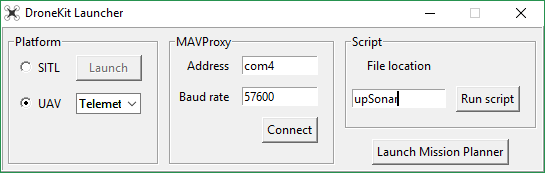
\includegraphics[width=\textwidth]{./figures/GUIwin.png}
		\caption{Windows version}
	\end{subfigure}
	~\\[1ex]
	\begin{subfigure}[b]{0.7\textwidth}
		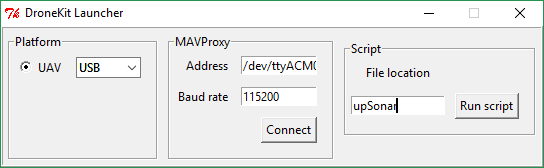
\includegraphics[width=\textwidth]{./figures/GUIlinux.png}
		\caption{Linux version}
	\end{subfigure}

	\caption{Graphical User Interface}
	\label{fig:gui}
\end{figure}

As it can be seen, the two versions have minimal differences.
Mainly, the Windows version, which was used in the early testing phases, provides the options of launching the SITL simulator as well as the Mission Planner GCS software for in-depth analysis of the incoming data (the bottom branch in Figure \ref{fig:mavproxy}).
Also, both versions autocomplete the MAVproxy fields according to the system they are run from, minimising errors and avoiding the memorisation of parameters by the pilot.


\section{Hardware implementation}
